\chapter{肌肉骨骼的几何学} \label{chap:chap6}


给我一个支点,用一根杠杆,我就能撬动整个世界。

\begin{flushright}
	——阿基米德
\end{flushright}


\begin{figure}[!htb]
	\centering
	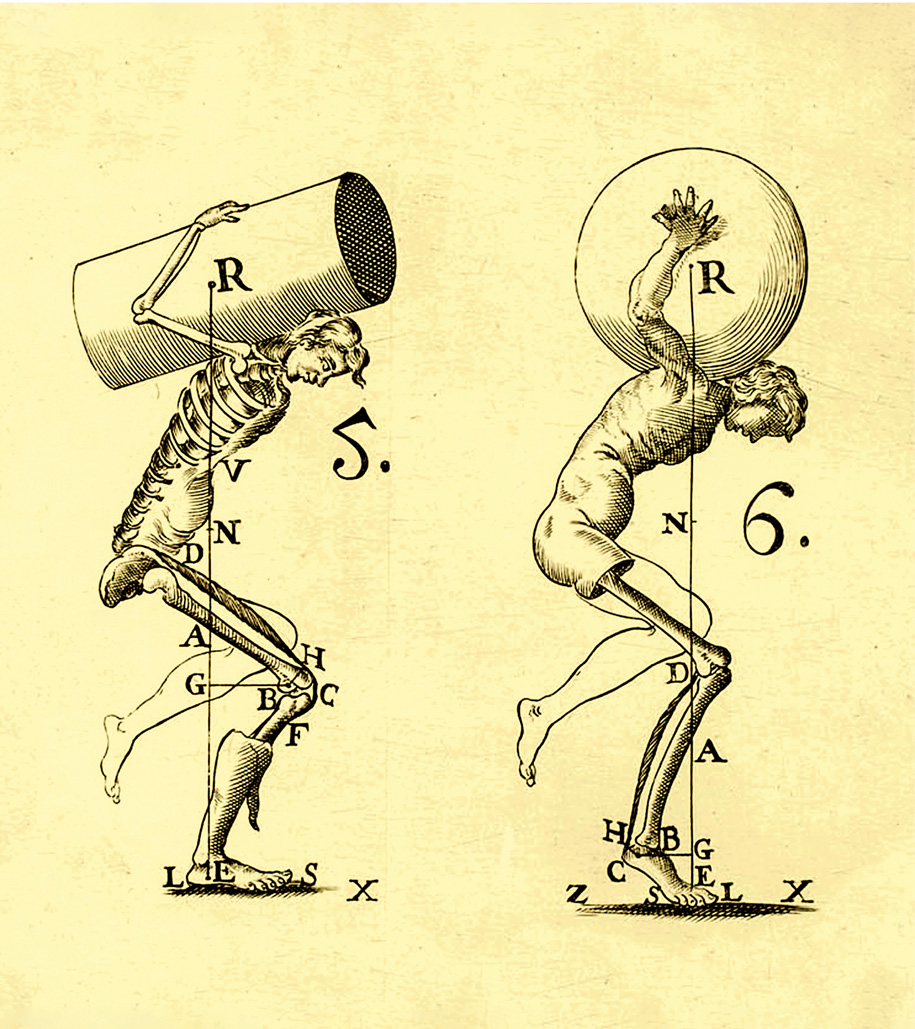
\includegraphics[width=1.0\linewidth]{chap6/6_0}
	% 加星号(*)表示不加编号
	\caption*{ \label{fig:6_0}}
\end{figure}


我读研究生的时候,我的一位导师是尤金$\cdot$布莱克,他是斯坦福医院骨科主任,也是脑瘫骨科治疗书籍的作者。
脑瘫是儿童最常见的残疾原因之一,会影响行走和保持平衡的能力。
脑瘫患者通常会形成一些独特的步态(例如蹲伏步态),这种步态效率低下且费力。


很多情况下,手术延长腿筋可以改善蹲伏步态。
但并非总是如此!
我问布莱克医生,他是如何决定是否延长某个病人的腿筋。
他告诉我,当肌肉“太紧”时,他会进行延长。
他通过观察孩子躺在他的检查床上时,肌肉能被拉伸到什么程度来评估肌肉的紧绷程度。
我走访了不同的医院,发现他们实施手术的标准并不一致。
我想,一定有更好的方法来确定哪些孩子会受益,哪些孩子不会。
问题仅仅是腿筋太短,还是还有其他问题无法通过延长肌肉来解决?


我们在第~\ref{chap:chap4}~章和第~\ref{chap:chap5}~章开始开发的计算机模型非常适合回答这些问题。
在对人体进行不可逆的手术之前,或许我们可以在计算模型上模拟手术。
但我们首先需要在这些模型中添加一些内容:
肌肉与骨骼相互作用以产生全身运动的方式。


我们首先要说明的是,肌肉通过向骨骼施加力量来产生运动。
然而,这里有一个微妙之处。
例如,如果你的二头肌恰好附着在肘关节上,你就永远无法移动前臂。
相反,肌肉附着在距离解剖关节一定距离的骨骼上,这样它们就有足够的杠杆作用来移动四肢(如果不是整个世界的话)。
这种杠杆作用称为肌肉的机械优势或力臂。
通过增加肌肉在骨骼上的附着点与关节旋转轴之间的距离,可以增加力臂。
其效果类似于将门把手放置在远离铰链的位置以便于打开门。
肌肉的机械优势由骨骼几何形状、身体姿势和肌肉作用线的路径决定。
我们将这些特征统称为肌肉骨骼几何形状。


正如我们将在本章中看到的,肌肉的机械优势与其在体内的功能密切相关。
因此,不同学科的科学家和临床医生都在研究肌肉骨骼几何学。
古生物学家研究已灭绝动物骨骼化石的形状,以确定肌肉的附着位置,并推断这些动物可能的运动方式。
生物力学家研究世界级运动员的肌肉骨骼几何学,以确定哪些特征使得他们能够取得优异的成绩。
外科医生可以应用肌肉骨骼模型来改善脑瘫患者的生活。


我们将从一个简单的例子开始,但它能让我们更好地理解这些模型的工作原理。
问题是:站立不动需要多大的努力?
将重心放在前脚掌上站立不动,还是将重心集中在双脚中部站立不动,哪个更难?



\section{肌肉机械优势}

为了回答这些问题,我们考虑进行二维静态分析,以了解单块踝关节跖屈肌在安静站立时维持身体直立所需的力量。
我们将身体建模为一个倒立摆,假设身体的整个重量由一条腿支撑,并比较 2 种情况。
在第一种情况下,人体站立时,其重量均匀分布在脚上,压力中心位于脚跟和脚趾之间的中间位置(图~\ref{fig:6_1},左)。
在第二种情况下,人体向前倾斜,压力中心移向脚趾。


\begin{figure}[!htb]
	\centering
	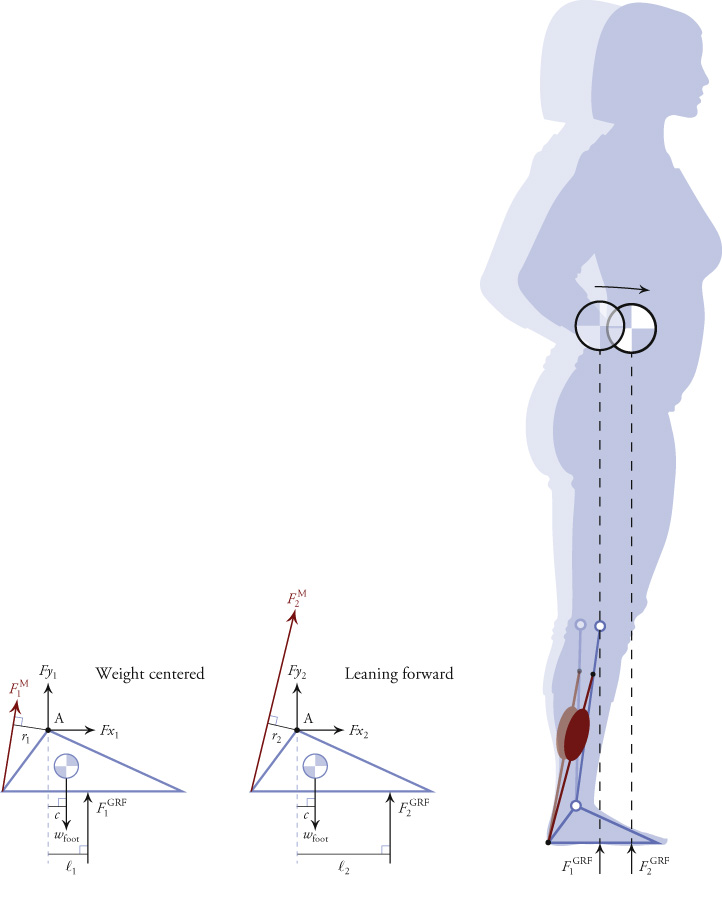
\includegraphics[width=0.9\linewidth]{chap6/6_1}
	\caption{自由体图(左图)和模型(右图)用于估计人处于直立姿势($F_1^M$)和前倾姿势($F_2^M$)时的跖屈肌力量。 \label{fig:6_1}}
\end{figure}


我们首先绘制每个场景下足部的自由体受力图,并将其与身体其他部位分离,以此开始分析。
我们将足部表示为一个三角形,并假设踝关节位于三角形的上顶点 A。
根据阿基米德杠杆定律,我们能够直立而不向前或向后倾倒,这意味着踝关节的力矩总和为零:
%
\begin{equation}
	\sum M_A = F_i ^{\text{GRF}} l_i 
				- w_\text{foot} c
				- F_i ^M r_i
				= 0
	\label{eq:6_1}
\end{equation}
%
索引 $i$ 代表两种情况:1 和 2,即人站立时重心集中在脚上,身体前倾。
重新排列此方程,我们可以计算出肌肉必须产生的力量:
%
\begin{equation}
	F_i ^M = 
		\frac{
			F_i ^{\text{GRF}} l_i
			- w_\text{foot} c
		}{
			r_i
		}
	\label{eq:6_2}
\end{equation}


该方程表明,肌肉中的作用力 ($F_i^M$) 受地面反作用力 ($F_i ^{\text{GRF}}$) 和足部重量 ($w_\text{foot}$) 的大小以及系统几何形状的影响:压力中心的位置 ($l_i$)、足部质心的位置 ($c$),以及值得注意的是从踝关节中心到肌肉力矢量的垂直距离 ($r_i$)。
距离 $r_i$ 定义了肌肉力矩臂。
力矩臂较小的肌肉必须施加更大的力才能产生与力矩臂较大的肌肉相同的关节力矩。
我们说力矩臂较大的肌肉具有更大的机械优势。


表~\ref{tab:6_1}~显示了每种情景下每个变量的实际量。
在第一种情景下,肌肉中的力量大致等于地面反作用力的大小(由于人处于静态平衡状态,因此等于体重)。
在第二种情景下,只需将压力中心向前移动 3 厘米,肌肉力量就会加倍。


\begin{table}[htbp]
	\caption{2 种情况下站立时肌肉力量的计算} \label{tab:6_1} \centering
	\begin{tabular}{ccccccc} % l水平左居中,c水平居中
		\toprule
		场景 & $F_i^{\text{GRF}}$ & $w_\text{foot}$ & $l_i$ & $c$ & $r_i$ & $F_i^M$ \\
		\midrule
		重心($i=1$) & 600牛 &  7.8牛 & 5厘米 & 1厘米 & 5厘米 & 598牛 \\
		\midrule
		向前倾($i=2$) & 600牛 &  7.8牛 & 8厘米 & 1厘米 & 4厘米 & 1198牛 \\
		\bottomrule
	\end{tabular}
\end{table}


请注意,我们平衡了踝关节周围的力矩来计算肌肉力(公式~\ref{eq:6_2})。
如果我们平衡水平和垂直方向的力,就可以计算出关节反作用力的 2 个分量($F_{x_i}$ 和 $F_{y_i}$)。
我们发现,即使在安静站立时,垂直力($F_{y_i}$)也约为体重的 2-3 倍。
由于肌肉的力臂通常较小,因此存在较大的关节内部接触力;
因此,即使在进行看似毫不费力的任务(例如静止站立或慢行)时,也可能需要较大的肌肉力。


上述示例将力学的基本概念应用于仅涉及一块肌肉的简单二维静态分析。
在下一节中,我们将对力臂进行更正式的工程定义,使其更广泛地应用于三维问题。



\section{肌肉力臂的定义}

在我们对肌肉骨骼几何结构的分析中,我们假设肌肉-肌腱单元可以建模为无摩擦、可伸缩的线,它们附着在骨骼上并缠绕在解剖结构周围。
尽管生物肌肉由数千条纤维组成,每条纤维都有独特的三维路径,但我们通常将肌肉表示为沿着从一个附着点到另一个附着点的路径作用的单一拉力。
该路径决定了肌肉力的作用点以及作用方向。
肌肉产生的力矩($ \underline{M} $)可以按如下方式计算(见图~\ref{fig:6_2}):


\begin{figure}[!htb]
	\centering
	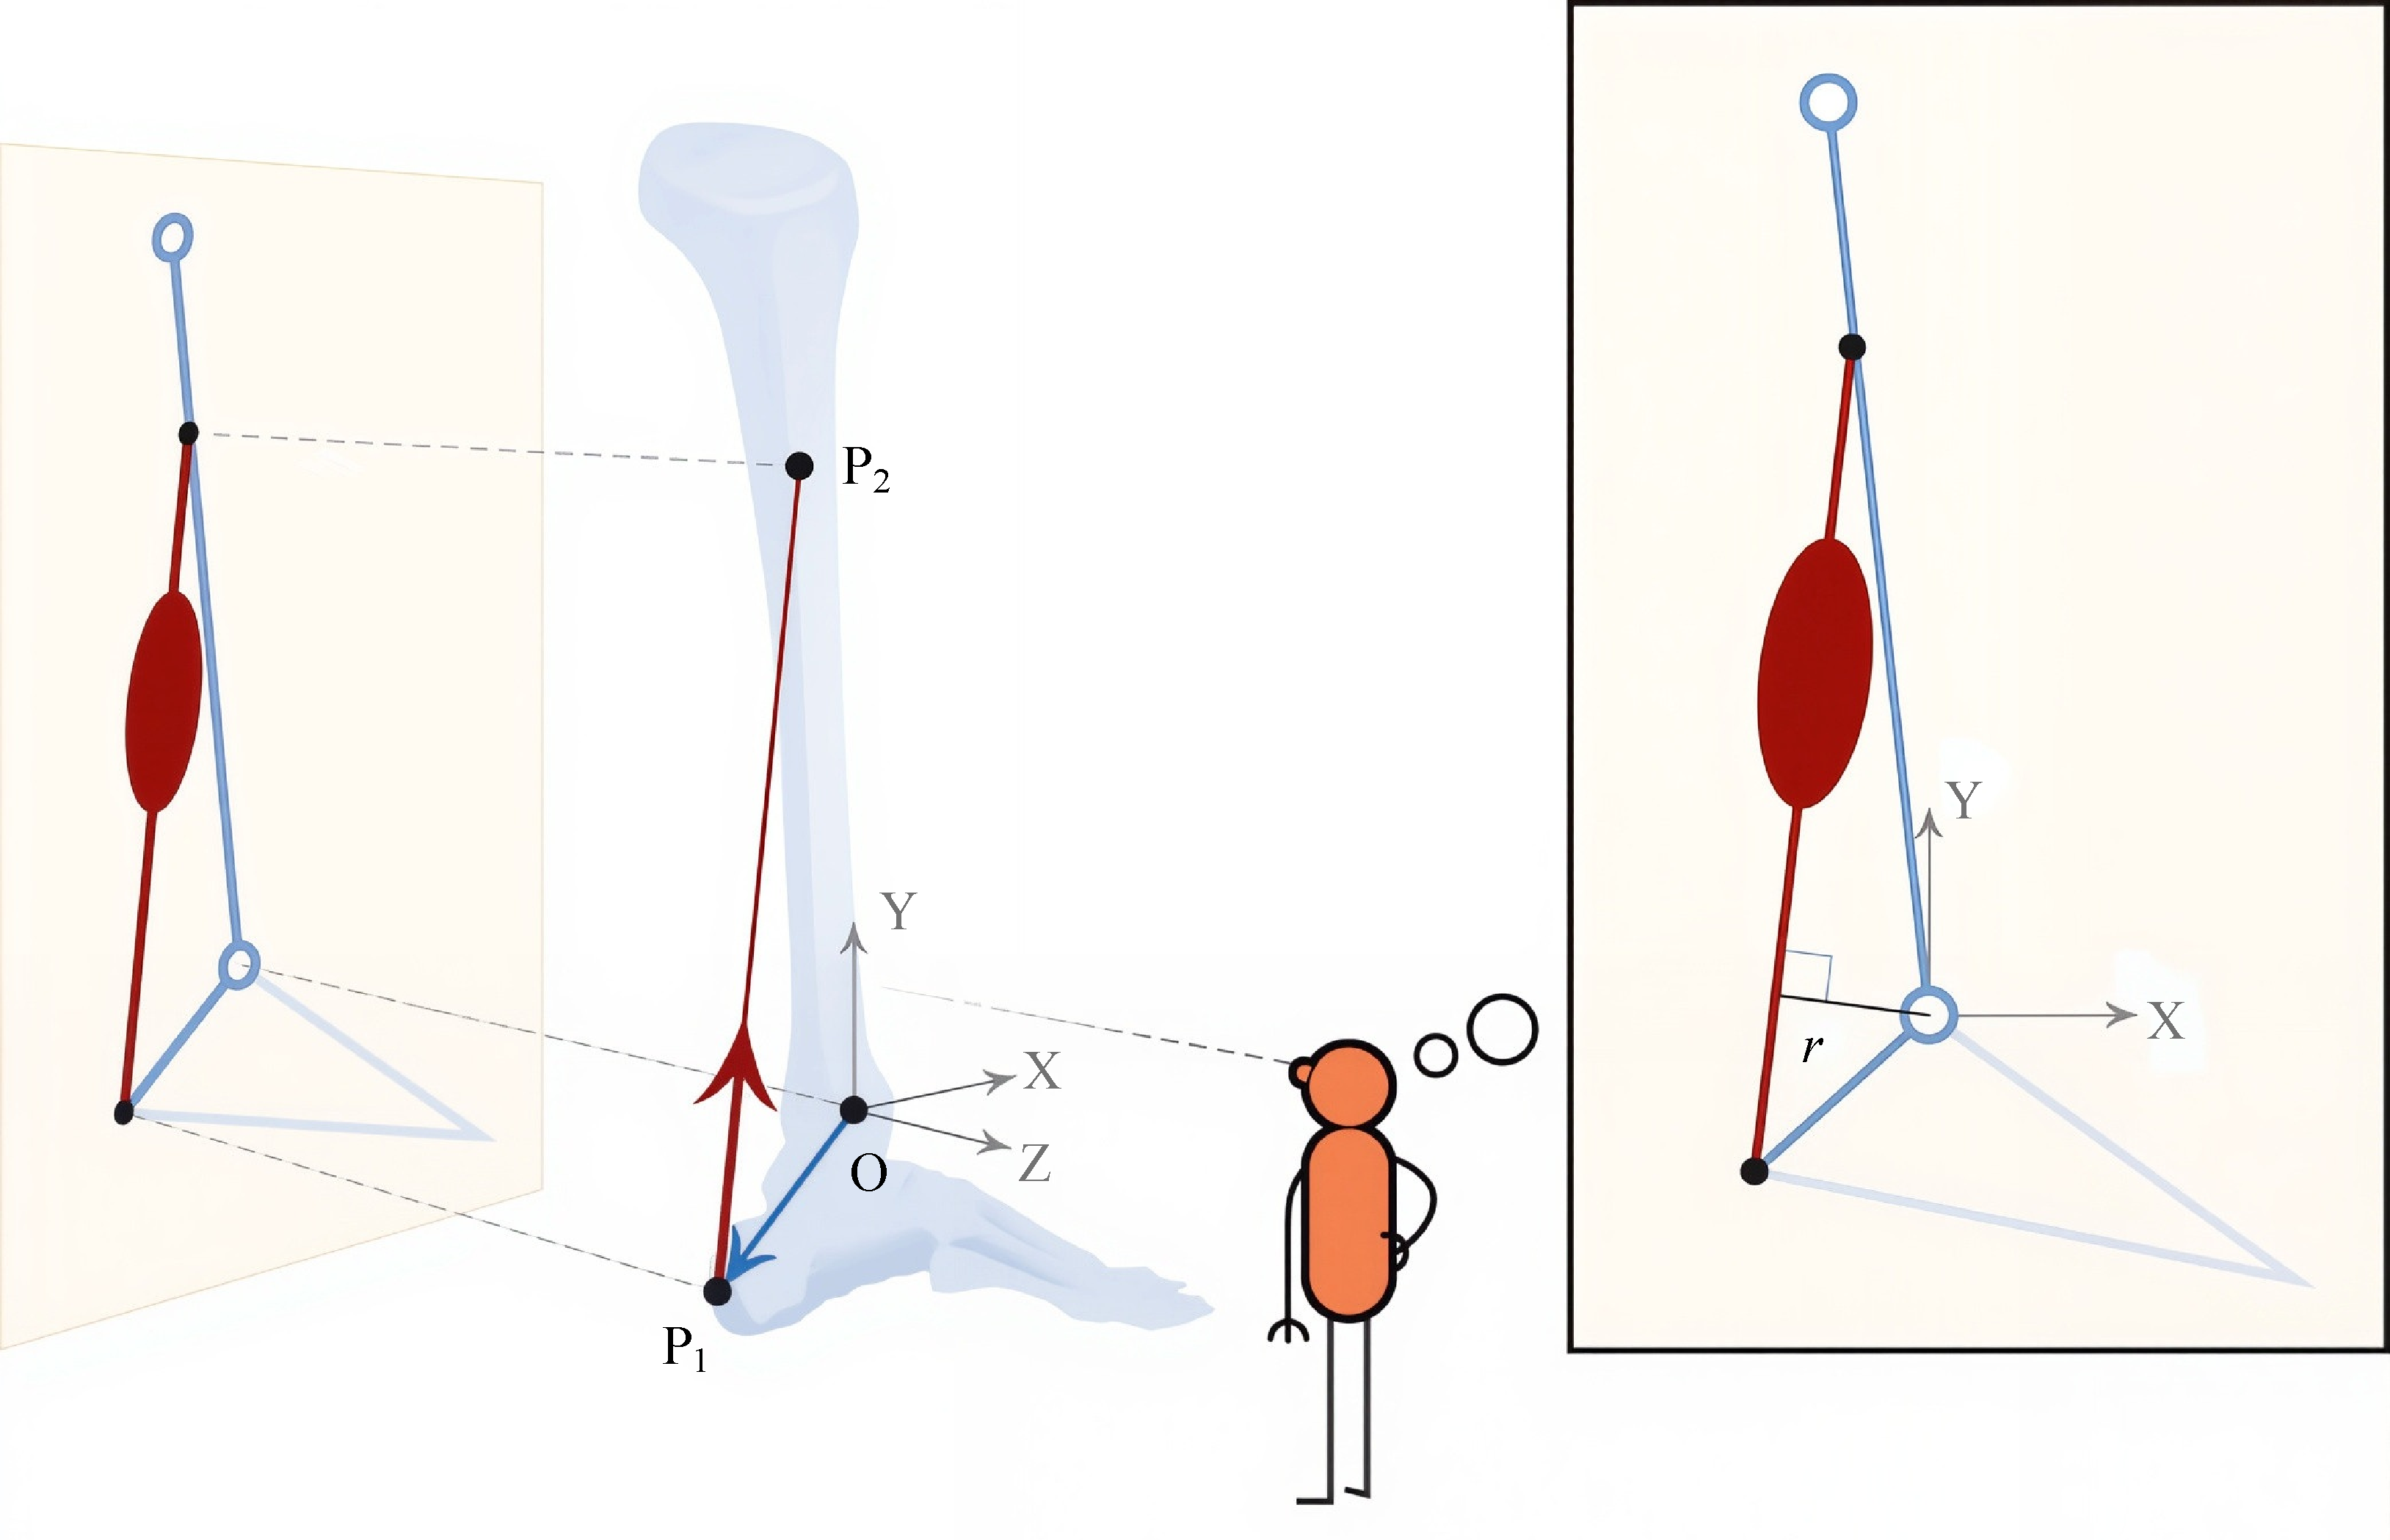
\includegraphics[width=0.9\linewidth]{chap6/6_2}
	\caption{与点 $O$ 处产生力矩有关的力矩臂 $r$ 的定义。 \label{fig:6_2}}
\end{figure}


\begin{equation}
	\underline{M} = \underline{r} \times \underline{F}
	\label{eq:6_3}
\end{equation}
%
其中,“$\times$”表示向量叉积。
点$O$表示关节的旋转中心,向量表示在点$P_1$施加的肌肉力的大小和方向,是从$O$到肌肉作用线上任意一点的向量。


如图~\ref{fig:6_2}~所示,直线肌肉模型的一个吸引人的特性是,$\underline{r}$ 可以从 $O$ 点画到 $P_1$ 点,或者画到 $P_2$ 点,或者画到肌肉作用线上的任何其他点。
在所有情况下,公式~\ref{eq:6_3}~中的叉积结果都相同。
肌肉产生的力矩 ($\underline{M}$) 是一个矢量,但通常更方便地获取标量。
在本例中,我们将公式~\ref{eq:6_3}~投影到 Z 轴上:
%
\begin{equation}
	M_z = ( \underline{r} \times \underline{F} \cdot \hat{z} )
	\label{eq:6_4}
\end{equation}
%
其中“$\cdot$”表示向量点积,$\hat{z}$ 是沿Z轴(与力矩$M_z$相关的旋转轴)的单位向量。
我们通过用肌肉力的大小($r$)对$M_z$进行归一化来定义肌肉的力臂($ \Vert \underline{F} \Vert $):
%
\begin{equation}
	r \triangleq 
		\frac{
			\underline{r} \times \underline{F}
		}{
			\Vert \underline{F} \Vert
		}
		\cdot
		\hat{z}
	\label{eq:6_5}
\end{equation}


记住,$r$ 表示从肌肉作用线到关节旋转中心的垂直距离。
在图~\ref{fig:6_3}~中,您可以看到如何通过踝关节的磁共振成像 (MRI) 扫描来估算这个距离。
这里我们必须假设踝关节的旋转轴 $\hat{z}$ 垂直于图像平面。
如果踝关节相对于扫描仪倾斜,那么我们对 r 的估计将不准确。
出于这个原因,并且由于我们并非总是有 MRI 扫描可用,我们将在下一节介绍另一种估算 $r$ 的策略。


\begin{figure}[!htb]
	\centering
	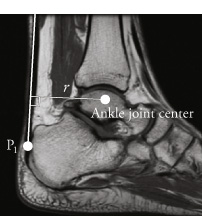
\includegraphics[width=0.4\linewidth]{chap6/6_3}
	\caption{通过磁共振图像估算肌肉力臂。
		MRI 图片由 Alex Frietas 提供。 \label{fig:6_3}}
\end{figure}


当关节角度变化时,肌肉作用线与旋转轴之间的垂直距离也会发生变化(图~\ref{fig:6_4})。
因此,肌肉的力臂会随着关节角度的变化而变化。
对于许多肢体肌肉而言,该函数在运动范围的中间附近达到峰值;
然而,不同肌肉之间的这种关系差异很大,如果我们要准确地表征力臂,就必须对其进行测量。


\begin{figure}[!htb]
	\centering
	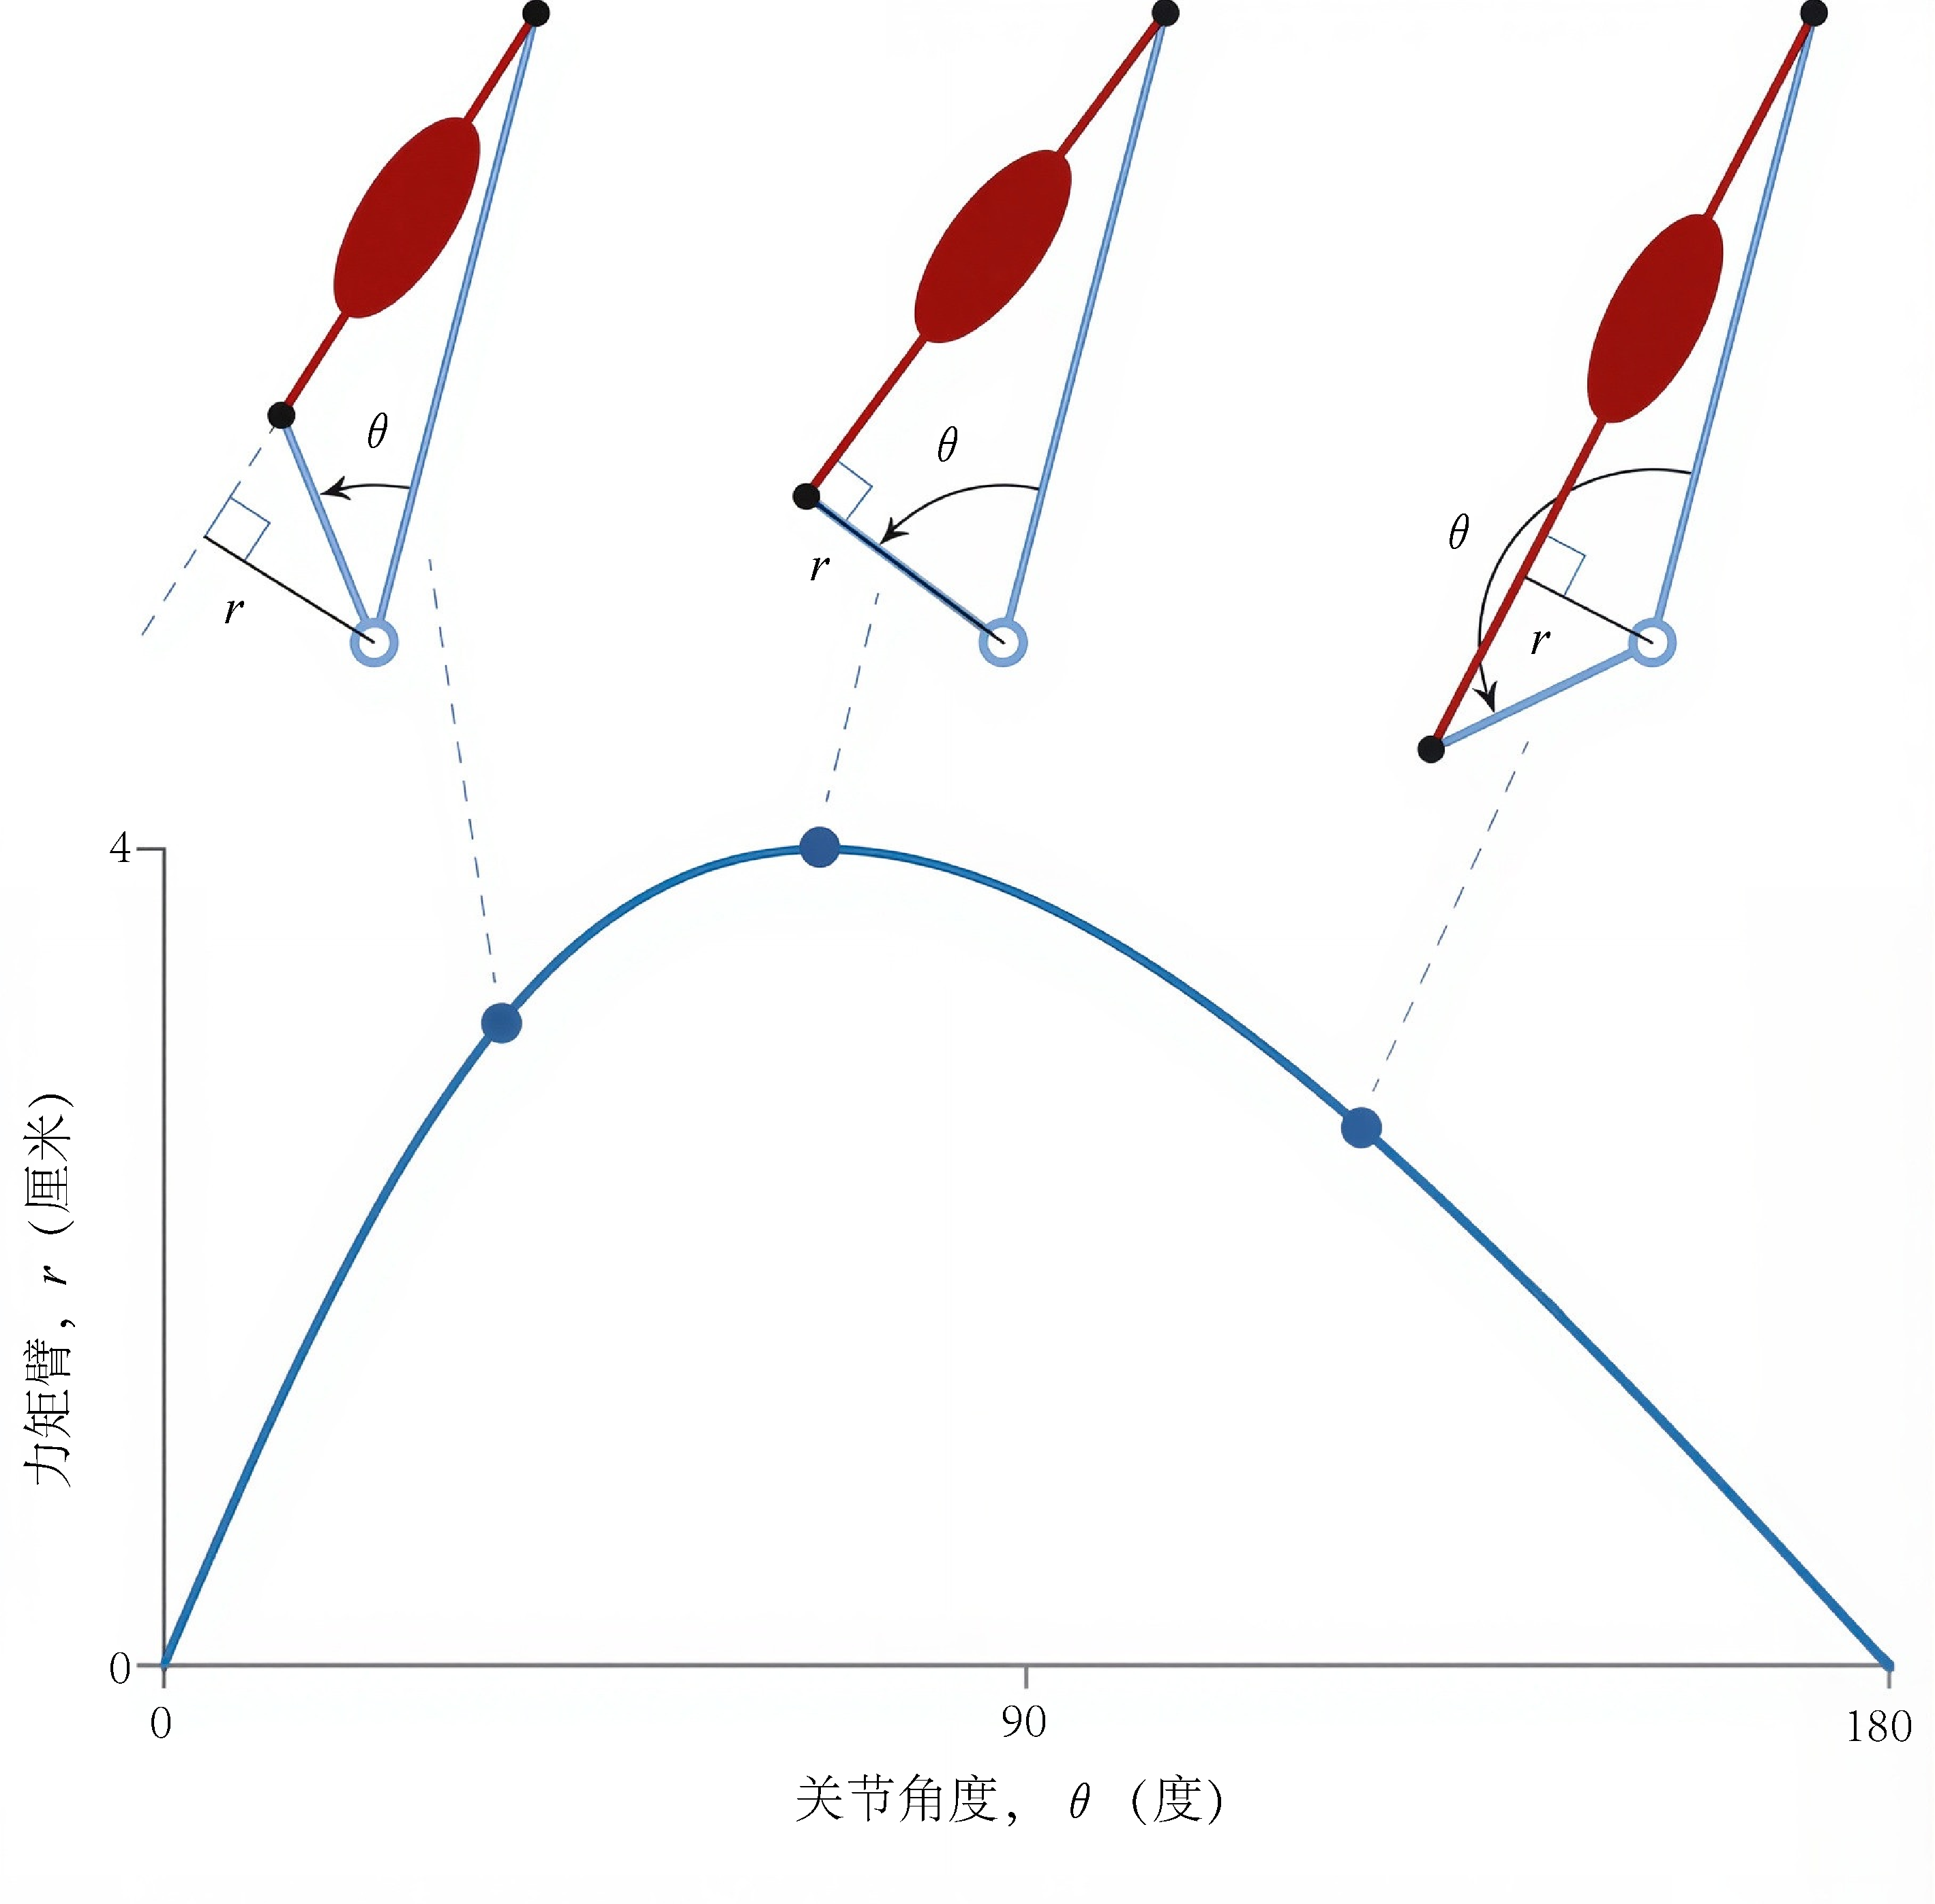
\includegraphics[width=0.8\linewidth]{chap6/6_4}
	\caption{演示肌肉的力臂 ($r$) 如何取决于它跨越的关节的角度 ($\theta$)。 \label{fig:6_4}}
\end{figure}


\section{力臂的肌腱偏移定义}

现在我们介绍力臂的第二个定义:肌腱偏移定义。
在某些假设下,该定义在数学上与图~\ref{fig:6_3}~中描述的解剖学定义等价;
然而,肌腱偏移定义提供了宝贵的概念见解。


考虑图~\ref{fig:6_4}~所示的系统,其中肌肉路径用线段表示。
该表示基于三个假设:
(1)肌肉的路径与肌肉力量无关(对于收缩时明显隆起的肌肉,情况可能并非如此);
(2)肌肉的路径可以由一系列线段定义(对于附着点较宽或路径几何形状复杂的大型肌肉,情况可能并非如此);
(3)肌肉-肌腱单元在邻近结构上滑动时不会产生摩擦(对于通过结缔组织附着于邻近肌肉的肌肉,情况可能并非如此)。


正如 An 等人\cite{an1984determination}所述,肌腱偏移定义源于将虚功原理应用于肌肉-关节系统。
虚功原理指出,对于一组无穷小的“虚位移”(时间保持不变时发生的假想位移),作用于处于静态平衡状态的系统上的所有力和力矩所做的总功为零。
肌肉所做的虚功 ($\delta w$) 定义为肌肉产生的力 ($F^M$) 与肌肉-肌腱单元的虚平移位移 ($\delta l^{MT}$) 的乘积:
%
\begin{equation}
	\delta w = F^M \delta l^{MT}
	\label{eq:6_6}
\end{equation}


为了使作用于该系统的所有力和力矩所做的总功为零,肌肉所做的虚功必须与外部力矩所做的虚功相平衡,定义如下:
%
\begin{equation}
	\delta w = M \delta \theta
	\label{eq:6_7}
\end{equation}
%
其中$\delta \theta$是关节的虚拟旋转位移。
使公式~\ref{eq:6_6}~和~\ref{eq:6_7}~的右边相等,可以平衡肌肉所做的虚拟功和外部力矩所做的虚拟功;代入公式~\ref{eq:6_3},可以得到以下关系:
%
\begin{equation}
	\begin{aligned}
		M \delta \theta & = F^M \delta l^{MT} \\
		r F^M \delta \theta & = F^M \delta l^{MT} \\
		r & = \frac{\delta l^{MT}}{\delta \theta}
	\end{aligned}
	\label{eq:6_8}
\end{equation}


最后,当虚拟位移趋于 0 时,我们取极限,此时该方程采用偏导数的形式:
%
\begin{equation}
	r = \frac{\partial l^{MT}}{\partial \theta}
	\label{eq:6_9}
\end{equation}

公式~\ref{eq:6_9}~使我们能够使用肌腱位移法通过实验测量力矩臂。
在该方法中,当关节在一定范围内运动时,用位置传感器监测肌肉-肌腱单元的长度;同时记录关节角度。
因此,我们获得了肌肉-肌腱长度随关节角度变化的样本(图~\ref{fig:6_5},左)。
为了根据这些数据确定力矩臂和关节角度之间的关系,我们可以简单地计算肌肉-肌腱长度对关节角度(以弧度为单位)的导数,如公式~\ref{eq:6_9}~所述。
表~\ref{tab:6_2}~中显示的数据和图~\ref{fig:6_5}~中的相应图表演示了如何使用中心差分法计算肌肉力矩臂作为关节角度的函数。
请注意,如果我们想使用图~\ref{fig:6_3}~所示的“解剖”方法确定这种关系,我们需要对踝关节进行多次不同屈曲度的 MRI 扫描。


\begin{figure}[!htb]
	\centering
	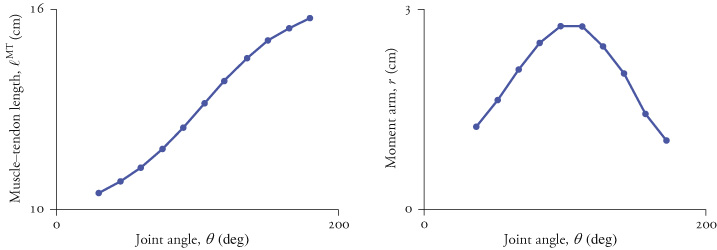
\includegraphics[width=1.0\linewidth]{chap6/6_5}
	\caption{使用数值导数计算的肌腱偏移数据和相应的力矩臂数据。
		这些曲线对应于表6.2所示的数据。 \label{fig:6_5}}
\end{figure}


\begin{table}[htbp]
	\caption{根据肌腱偏移数据计算力矩臂} \label{tab:6_2} \centering
	\begin{tabular}{cccccc} % l水平左居中,c水平居中
		\toprule
		$\theta$\text{(度)}$$ & $l^{MT}(\text{厘米})$ & $\Delta \theta($\text{度}$)$ & $\Delta l^{MT}(\text{厘米})$ & $\text{中点处的} \theta$(度) & $\text{力臂}(厘米)$ \\
		\midrule
		30 & 10.50 &    & & & \\
		\midrule
		45 & 10.82 &  $\pi / 12$  & 0.32 & 37.5 & 1.22 \\
		\midrule
		60 & 11.25 &  $\pi / 12$  & 0.43 & 52.5 & 1.64 \\
		\midrule
		75 & 11.80 &  $\pi / 12$  & 0.55 & 67.5 & 2.10 \\
		\midrule
		90 & 12.45 &  $\pi / 12$  & 0.65 & 82.5 & 2.48 \\
		\midrule
		105 & 13.17 &  $\pi / 12$  & 0.72 & 97.5 & 2.75 \\
		\midrule
		120 & 13.89 &  $\pi / 12$  & 0.72 & 112.5 & 2.75 \\
		\midrule
		135 & 14.53 &  $\pi / 12$  & 0.64 & 127.5 & 2.44 \\
		\midrule
		150 & 15.06 &  $\pi / 12$  & 0.53 & 142.5 & 2.02 \\
		\midrule
		165 & 15.44 &  $\pi / 12$  & 0.38 & 157.5 & 1.45 \\
		\midrule
		180 & 15.71 &  $\pi / 12$  & 0.27 & 172.5 & 1.03 \\
		\bottomrule
	\end{tabular}
\end{table}


我们和其他人测量了手臂和腿部许多肌肉的肌腱偏移,并利用这些数据估算了这些肌肉的力臂。
例如,温迪$\cdot$默里测量了肘部主要肌肉的肌腱偏移和力臂(图~\ref{fig:6_6})。
这些数据有助于测试肌肉骨骼系统计算机模型对人体几何形状的准确描述,并有助于确定描述个体间肌肉骨骼几何形状差异的规则。


\begin{figure}[!htb]
	\centering
	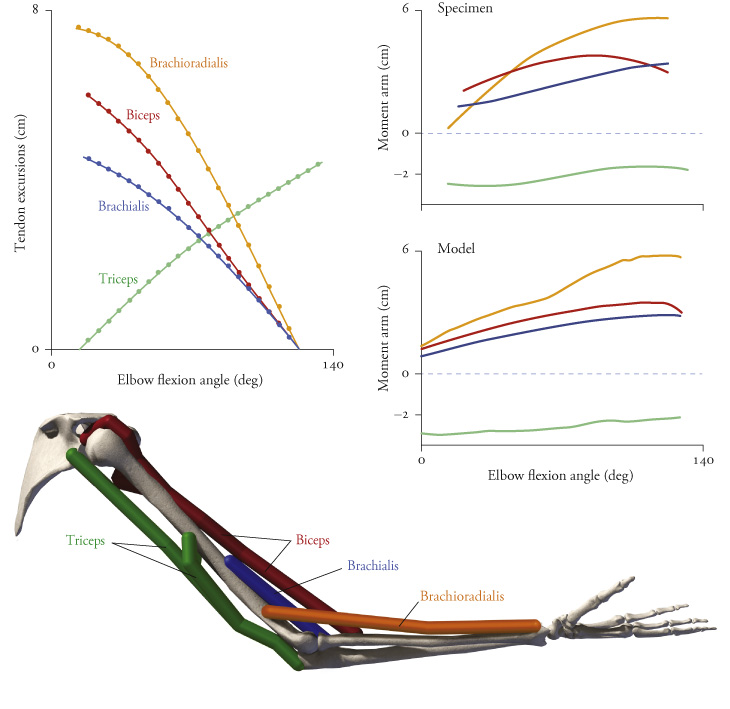
\includegraphics[width=1.0\linewidth]{chap6/6_6}
	\caption{肘部主要肌肉的肌腱偏移和力臂\cite{murray1995variation}。 \label{fig:6_6}}
\end{figure}


\section{肌肉力臂影响肌肉长度和速度}

力臂的肌腱偏移定义表明,在给定的关节运动范围内,如果肌腱单元的力臂较大,其长度变化也会较大。
由于肌肉的产力能力取决于其长度(这是力-长度关系的体现),因此,力臂较大的肌肉比力臂较小的肌肉在力-长度曲线上的作用范围更大(假设肌肉的最佳纤维长度相同;图~\ref{fig:6_7})。

\begin{figure}[!htb]
	\centering
	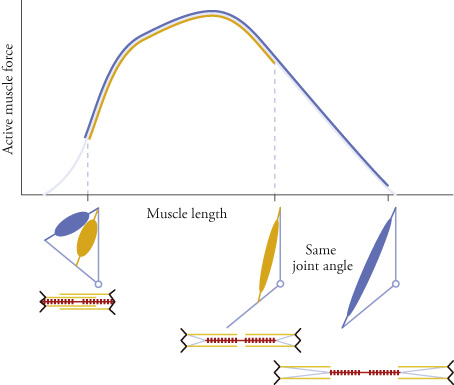
\includegraphics[width=0.7\linewidth]{chap6/6_7}
	\caption{两块肌肉具有相同的最佳纤维长度,但力臂不同,其长度变化量也不同,因此,在相同的关节角度范围内,其主动力-长度曲线的范围也不同。 \label{fig:6_7}}
\end{figure}


对于给定的关节角速度 ($\partial \theta / \partial t$),肌肉的力臂也会影响肌腱单元 ($v^{MT}$) 的速度。
可以通过首先将公式~\ref{eq:6_9}~乘以关节角速度,以数学方式检验 $v^{MT}$ 与 $v^{MT}$ 之间的关系:
%
\begin{equation}
	(
		\frac{\partial l^{MT}}{\partial \theta}
	)
	(
		\frac{\partial \theta}{\partial t}
	)
	=
	r \frac{\partial \theta}{\partial t}
	\label{eq:6_10}
\end{equation}


简化公式~\ref{eq:6_10},我们得到以下关系:
%
\begin{equation}
	\frac{\partial l^{MT}}{\partial t}
	=
	v^{MT}
	=
	r \frac{\partial \theta}{\partial t}
	\label{eq:6_11}
\end{equation}


公式~\ref{eq:6_11}~表明,对于给定的关节角速度,力臂较大的肌肉将比力臂较小的肌肉经历更高的速度。
这种关系具有重要的功能意义,因为肌肉力取决于肌肉速度,正如力-速度曲线所示(图~\ref{fig:6_8})。


\begin{figure}[!htb]
	\centering
	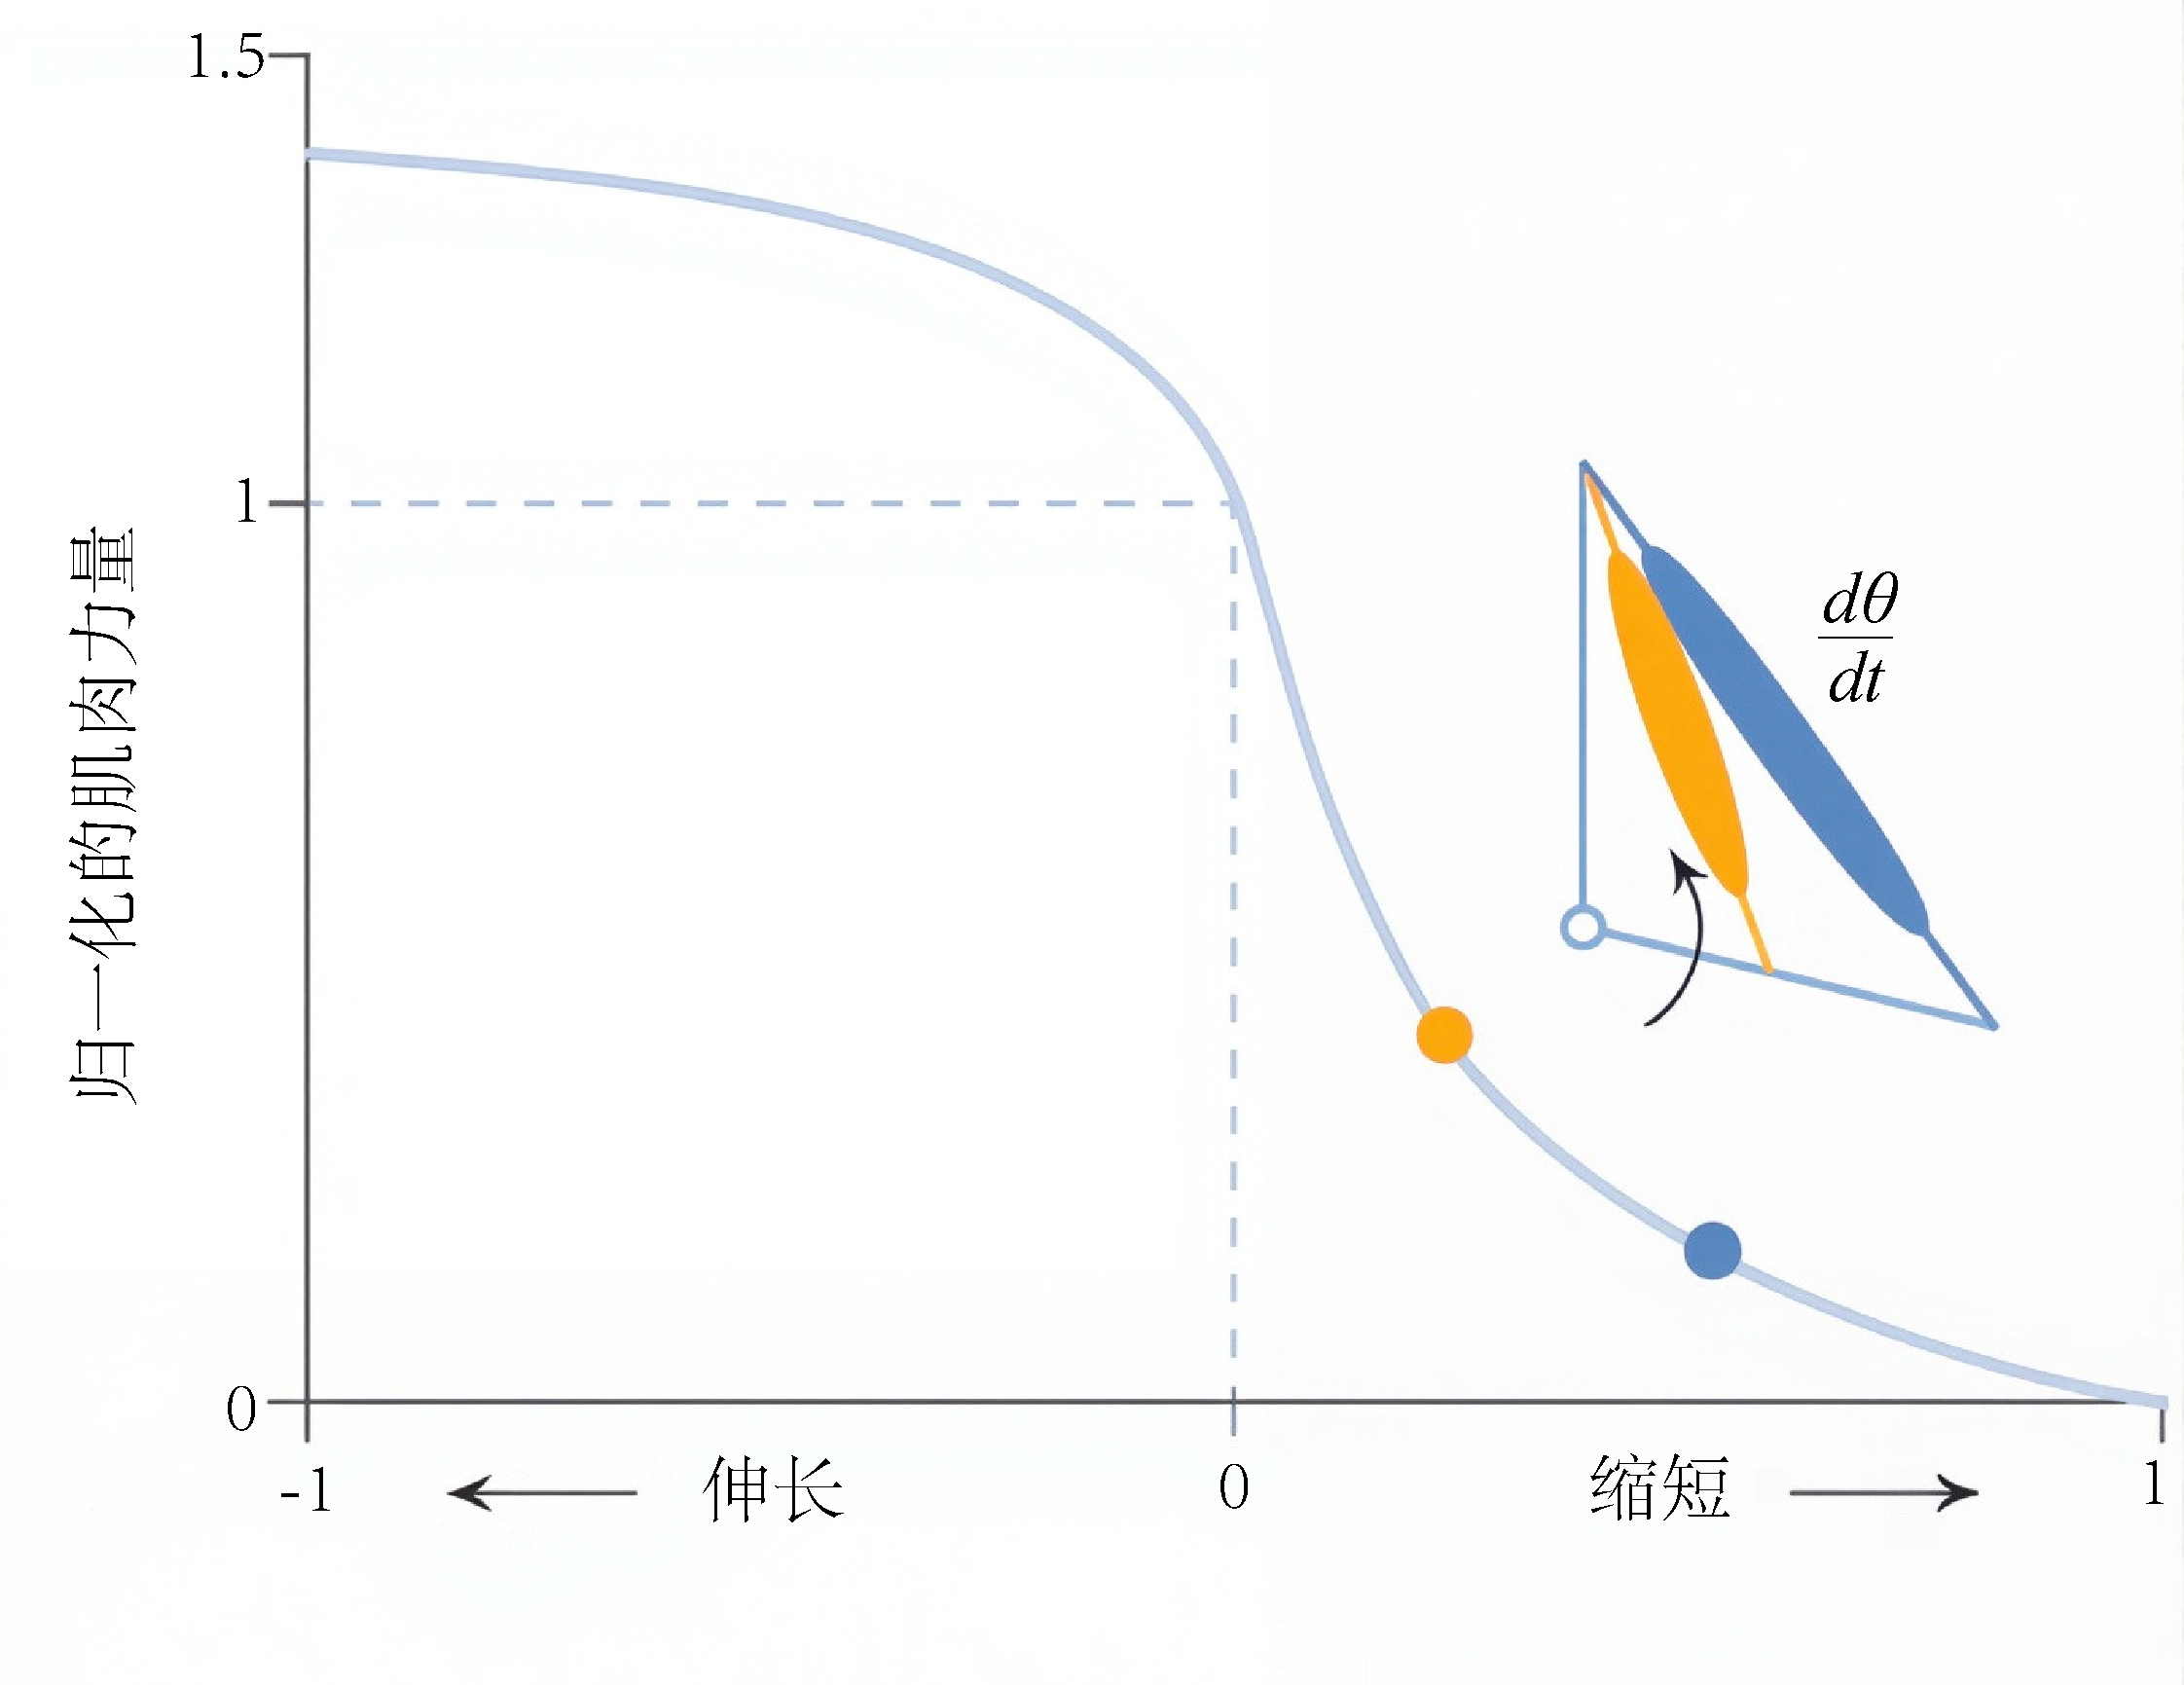
\includegraphics[width=0.6\linewidth]{chap6/6_8}
	\caption{力臂较大的肌肉(蓝色)的缩短速度会比力臂较小的肌肉(橙色)更快。
		由于力与速度的关系,力臂较大的肌肉的产力能力会较低。 \label{fig:6_8}}
\end{figure}


肌肉力矩臂对肌肉速度的影响表明,如果肌肉驱动承受高角速度的关节,那么较小的力矩臂和较长的肌肉纤维可能有益,因为这样可以降低肌肉纤维缩短的速度。
事实上,Sabrina Lee\cite{lee2009built}发现,与体型匹配的非短跑运动员相比,精英短跑运动员的跟腱力矩臂要小 25\%,踝关节肌肉纤维要长 11\%。
更长的肌肉纤维和较小的力矩臂使精英短跑运动员能够将跖屈肌纤维长度保持在更接近其最佳长度的水平,并在跑步的蹬地阶段踝关节快速跖屈时降低纤维缩短速度。
这些形态特征增加了跖屈肌的发力能力,从而使它们能够产生高速跑步所需的巨大力量。


除了比较不同个体的同一块肌肉之外,比较同一个体不同肌肉的能力以及它们如何受到力臂的影响也很有帮助。
增加肌肉的力臂会增加它能产生的最大力矩的大小,但也会增加它在特定运动中长度变化的量(和速率)。
当肌纤维达到其力-长度关系的极限时,较大的长度变化会导致肌肉在关节活动范围极限处的发力能力下降。
这两个现象在最大力矩和最大关节活动范围之间造成了权衡。
不同的肌肉会在可能的力臂范围内的不同点上运作,使每一块肌肉都适合执行一组特定的功能,并且共同使人体具有非凡的多功能性。


\section{多关节肌肉的力臂}

到目前为止,我们的分析仅限于仅跨越一个关节的肌肉,然而许多肌肉跨越多个关节,并且每个关节都有力臂。
例如,腘绳肌(腿筋之一)的半膜肌跨越髋关节和膝关节后方,因此在平面模型中有两个力臂(图~\ref{fig:6_9})。
事实上,即使一块肌肉只跨越一个关节,它也会在该关节的每个自由度上分别有一个力臂。
例如,臀大肌只跨越髋关节,它在髋关节伸展、髋关节外展和髋关节旋转时都具有力臂。
每个自由度的力臂可以用公式~\ref{eq:6_4}~计算。


\begin{figure}[!htb]
	\centering
	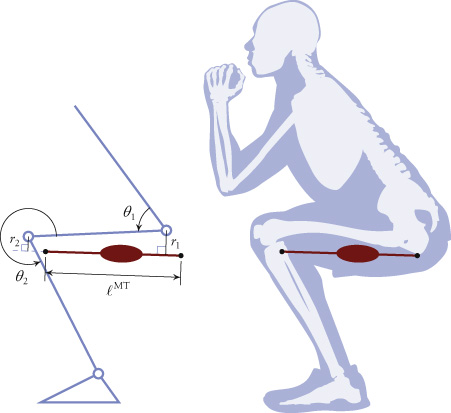
\includegraphics[width=0.8\linewidth]{chap6/6_9}
	\caption{腘绳肌在髋部和膝部后方交叉。
		图中所示的肌肉具有髋部伸展力臂 ($r_1$) 和膝部屈曲力臂 ($r_2$)。
		其长度 ($l^{MT}$) 和速度取决于关节角度 ($\theta_1$ 和 $\theta_2$) 以及角速度。 \label{fig:6_9}}
\end{figure}


肌肉在身体运动过程中长度的变化量取决于肌肉所跨越关节的位移以及肌肉相对于每个关节角度的力臂。
肌腱单元的速度取决于肌肉所跨越关节的角速度,同样也取决于肌肉相对于每个关节角度的力臂。
我们可以推广公式~\ref{eq:6_11},计算跨越 $n$ 个关节的肌腱单元 ($v^{MT}$) 的速度,如下所示:
%
\begin{equation}
	v^{MT} = 
		\sum_{i=1}^{n}
			r_i
			\frac{d \theta_i}{d t}
	\label{eq:6_12}
\end{equation}
%
其中 $r_i$ 是与第 $i$ 个自由度 ($\theta_i$) 对应的力矩臂。


正如我们在本章开头提到的,肌肉-肌腱长度和速度的计算可以指导运动障碍的治疗。
这可能对以蹲伏步态行走的脑瘫患者有所帮助,在这种情况下,膝盖的屈曲程度超过正常水平(图~\ref{fig:6_10},左)。
这种步态异常通常归因于限制膝关节伸展的“短”或“痉挛”腘绳肌,通常通过手术延长腘绳肌来治疗。
我和Allison Arnold与来自多家儿童医院的同事合作,研究了蹲伏步态患者的腘绳肌是否比正常人短,这表明他们可能适合接受腘绳肌延长手术。
我们检查了152名儿童的蹲伏步态,测量了他们的关节角度和步幅持续时间,然后使用计算机模型计算了整个步态周期内腘绳肌的肌肉-肌腱长度和速度。
我们将结果与 45 位未受损个体计算出的相同长度和速度进行了比较。
所有长度和速度均已标准化,以反映参与者的不同体型。
由此绘制的图表使我们能够区分腘绳肌峰值长度短于正常值的受试者和腘绳肌峰值速度慢于正常值的受试者。
例如,受试者 1 行走时腘绳肌长度明显短于正常值,而受试者 2 行走时腘绳肌速度明显慢于正常值(图~\ref{fig:6_10},右)。


\begin{figure}[!htb]
	\centering
	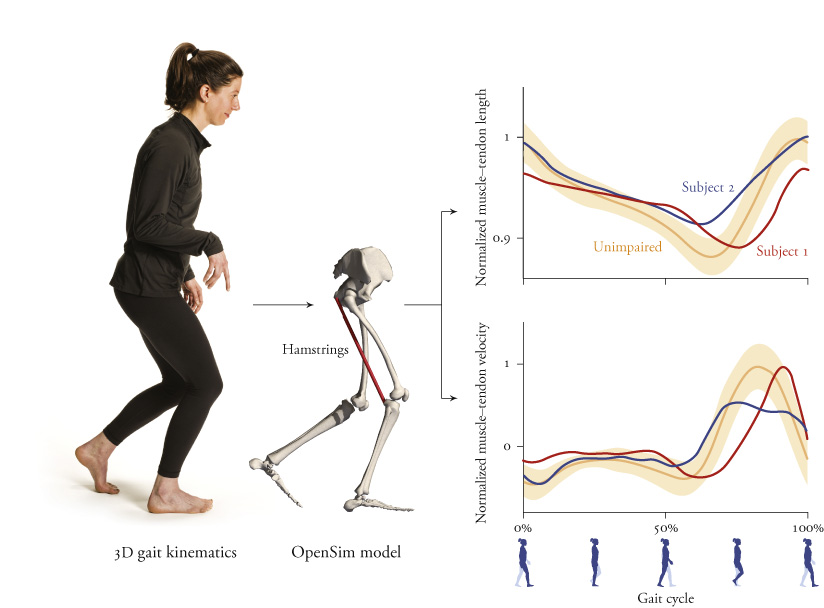
\includegraphics[width=1.0\linewidth]{chap6/6_10}
	\caption{肌肉骨骼几何模型(中间)可用于计算步态过程中腘绳肌的肌腱长度和速度。
		右侧图表比较了两名蹲伏步态受试者的腘绳肌长度和速度,以及 45 名未受损个体的平均值(平均值±2 个标准差)\cite{arnold2006role}。 \label{fig:6_10}}
\end{figure}


分析腘绳肌的长度和速度可以判断哪些人适合接受腘绳肌手术。
我们分析的受试者中,约有三分之一的腘绳肌长度正常,行走速度也正常,这表明他们的肌肉并不太紧张,手术对他们没有好处。
约有三分之二的受试者的腘绳肌较短或速度较慢;这些患者更有可能从腘绳肌手术延长中获益。
虽然估算肌肉长度和速度只是难题的一部分,但这些数据为评估哪些肌肉应该接受手术延长提供了客观依据。
为了方便其他人进行这些评估,我的实验室提供了免费的肌肉骨骼几何模型和名为 OpenSim 的开源软件,用于分析肌肉骨骼力学。
这些工具目前已被许多医院用于辅助手术规划,欢迎您也使用它们。



\section{最大关节力矩的测量与建模}

前几节说明了力臂会随着关节角度而变化,肌肉力量也是如此。
我们还看到,一块肌肉可以驱动多个关节。
反之亦然——每个关节都由多块肌肉驱动,每块肌肉都有各自的结构和几何形状。


驱动关节的肌肉成对出现:主动肌使关节向一个方向旋转,拮抗肌使关节向相反方向旋转。
例如,在行走过程中,小腿前侧的胫骨前肌产生力量,控制足部在触地后下沉至地面(图~\ref{fig:6_11},左)。
随后,小腿后侧的肌肉产生力量,使踝关节跖屈,并在步态周期的蹬地阶段产生地面反作用力(图~\ref{fig:6_11},右)。


\begin{figure}[!htb]
	\centering
	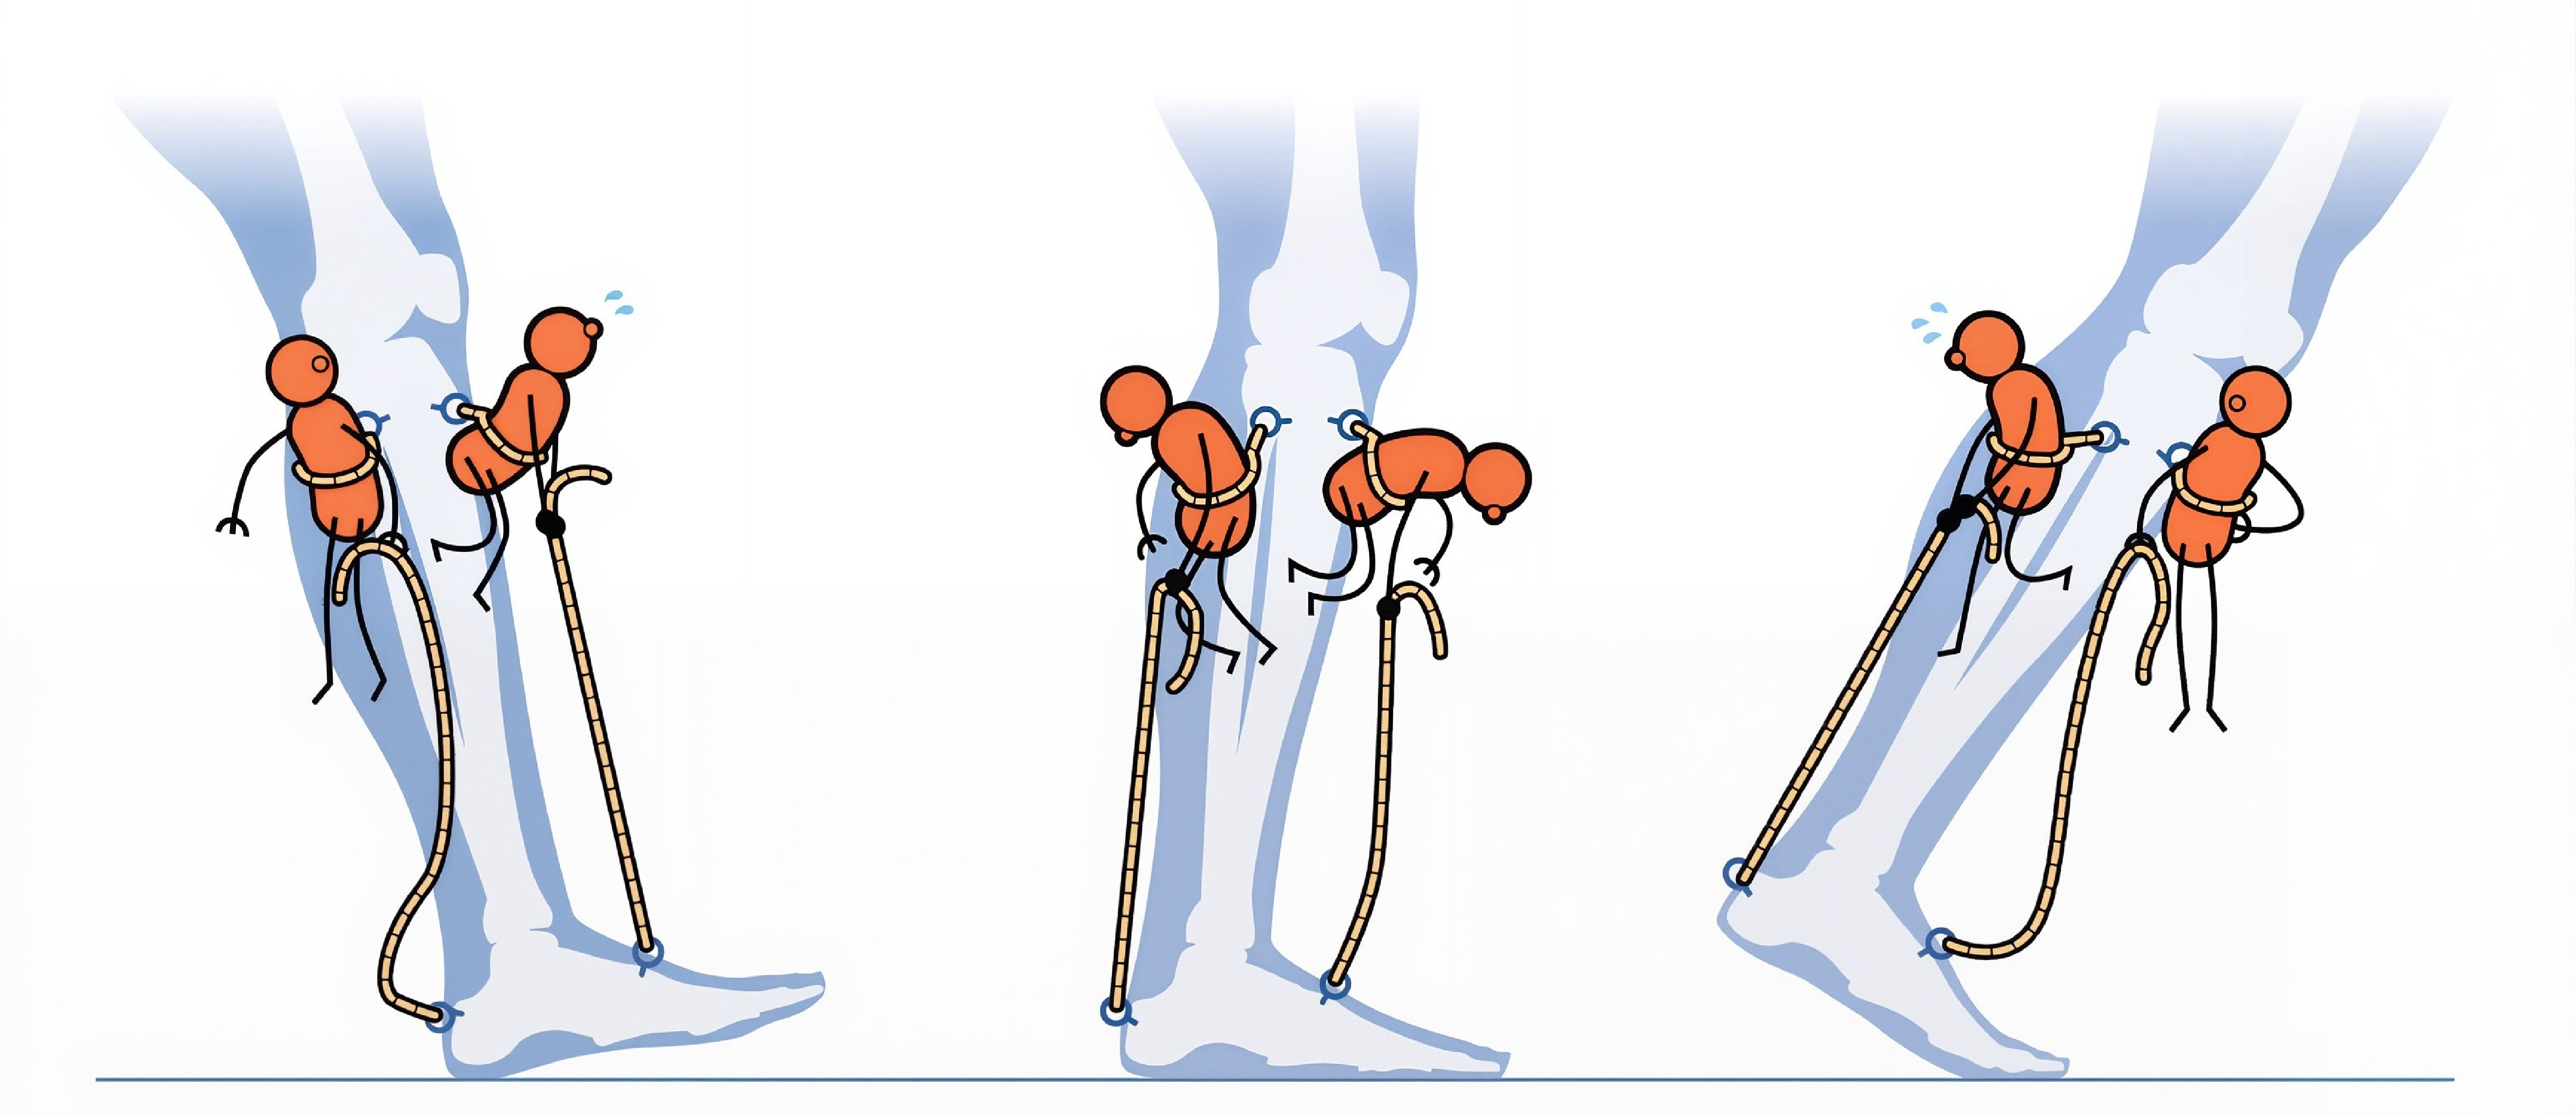
\includegraphics[width=1.0\linewidth]{chap6/6_11}
	\caption{骨骼肌通过拉动其所附着的骨骼来产生运动。
		主动肌和拮抗肌的力量会同步产生协调的运动。
		灵感源自 Verne Inman 的著作《人类行走》(1981 年)。 \label{fig:6_11}}
\end{figure}


这种安排的原因很简单:肌肉只能拉动(它们无法推动)。
乍一看,这似乎有悖常理,因为在日常用语中,我们经常谈论“推动”(包括在最后一段中提到的“蹬离阶段”)。
然而,如果你仔细思考,当我们所谓的“蹬离”时,哪些肌肉在做功,你会发现这些肌肉实际上在拉动。
脚的“蹬离”实际上是由小腿肌肉的紧张产生的。


虽然图~\ref{fig:6_11}~中只展示了两块肌肉,但主动肌和拮抗肌实际上可能是肌肉群。
例如,大腿中所谓的“股四头肌”实际上由四块独立的肌肉组成(前缀“quadri-”在拉丁语中意为“四”)。
在预测股四头肌或作用于关节的所有肌肉的最大力量时,我们需要考虑每块肌肉的结构和几何形状,并意识到肌肉总力矩会随着关节角度和角速度的变化而变化。


最大自主等长力矩通常由肌肉骨骼系统的计算机模型预测,但也可以使用测力计进行实验测量(图~\ref{fig:6_12})。
例如,为了测量肘屈肌的力量,受试者可以坐着,将其手腕连接到称重传感器上,以测量肢体施加的力。
在测量最大等长力量时,受试者的身体位置在实验过程中受到限制。
通常,在研究者观察受试者以确保他们只使用肘屈肌并施加最大力量的同时,会进行多次尝试以达到最大力矩。
然后,可以让受试者重新定位几次,以测量他们在一系列肘屈角度下的最大力量,如图~\ref{fig:6_12}~所示。


\begin{figure}[!htb]
	\centering
	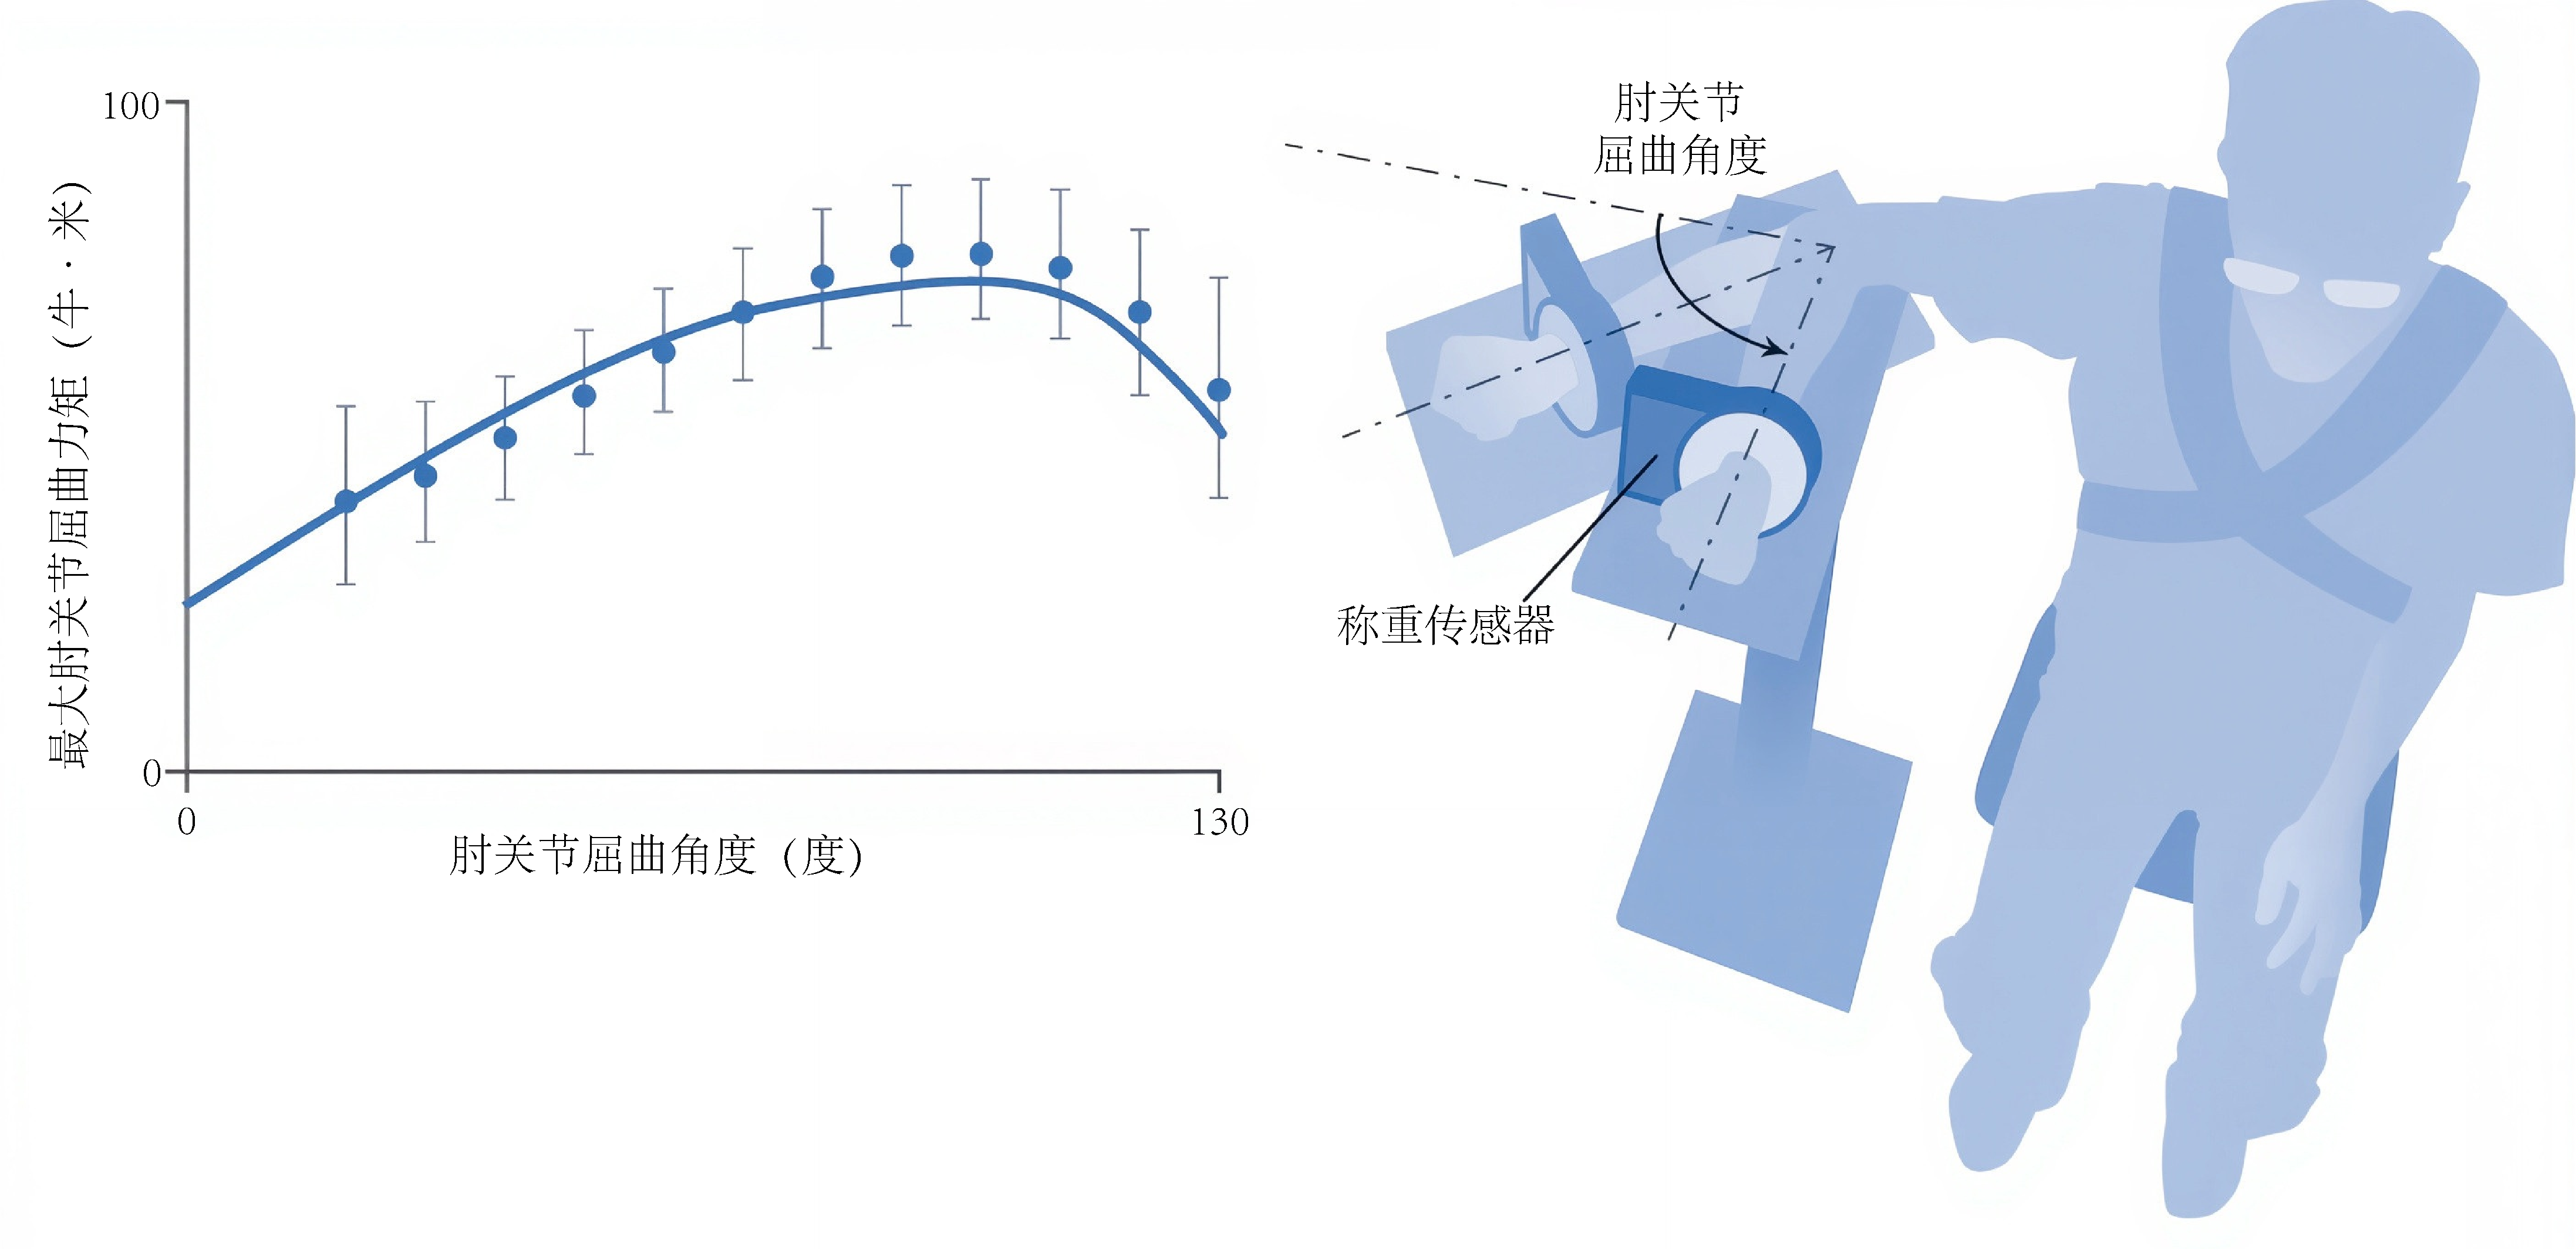
\includegraphics[width=1.0\linewidth]{chap6/6_12}
	\caption{测量肘屈肌产生的最大等长力矩。
		左侧数据由 Thomas Buchanan 等人\cite{buchanan1998muscular}收集,使用与右侧所示类似的实验装置进行测量。 \label{fig:6_12}}
\end{figure}


请注意,图~\ref{fig:6_12}~中所示的最大等长力矩会随肘部屈曲角度而变化。
该力矩由多块肌肉(例如肱二头肌、肱肌和肱桡肌;见图~\ref{fig:6_6})产生,由于每块肌肉的力臂和产力能力不同,因此每块肌肉产生的肘部屈曲力矩也会随肘部屈曲角度而变化。


为了更深入地探究这一概念,请参考图~\ref{fig:6_13},图中我们可以看到横跨单个关节的两块虚拟肌肉——“强肌”和“长肌”,其力矩臂、肌肉力和关节力矩相对于关节角度的示意图。
强肌纤维较短,PCSA 较大,力矩臂相对较小;长肌纤维较长,PCSA 较小,力矩臂较大。
对于每块肌肉,在给定关节角度下可产生的最大关节力矩是力矩臂与该角度下可产生的最大力的乘积(公式~\ref{eq:6_4})。
关节的总肌肉力矩是通过将两条力矩与角度曲线(每块肌肉一条)相加来计算的,从而得出关节的最大自主等长力矩。
请注意,在关节角度较小时,强肌产生的力矩最大;在关节角度较大时,长肌贡献了关节总力矩的大部分。
这两块肌肉协同工作,确保在整个运动范围内至少能产生适度的关节力矩。
临床上通常只测量关节总力矩(见图~\ref{fig:6_12})。
模型和模拟对于理解单个肌肉如何参与产生测量到的关节力矩至关重要。


\begin{figure}[!htb]
	\centering
	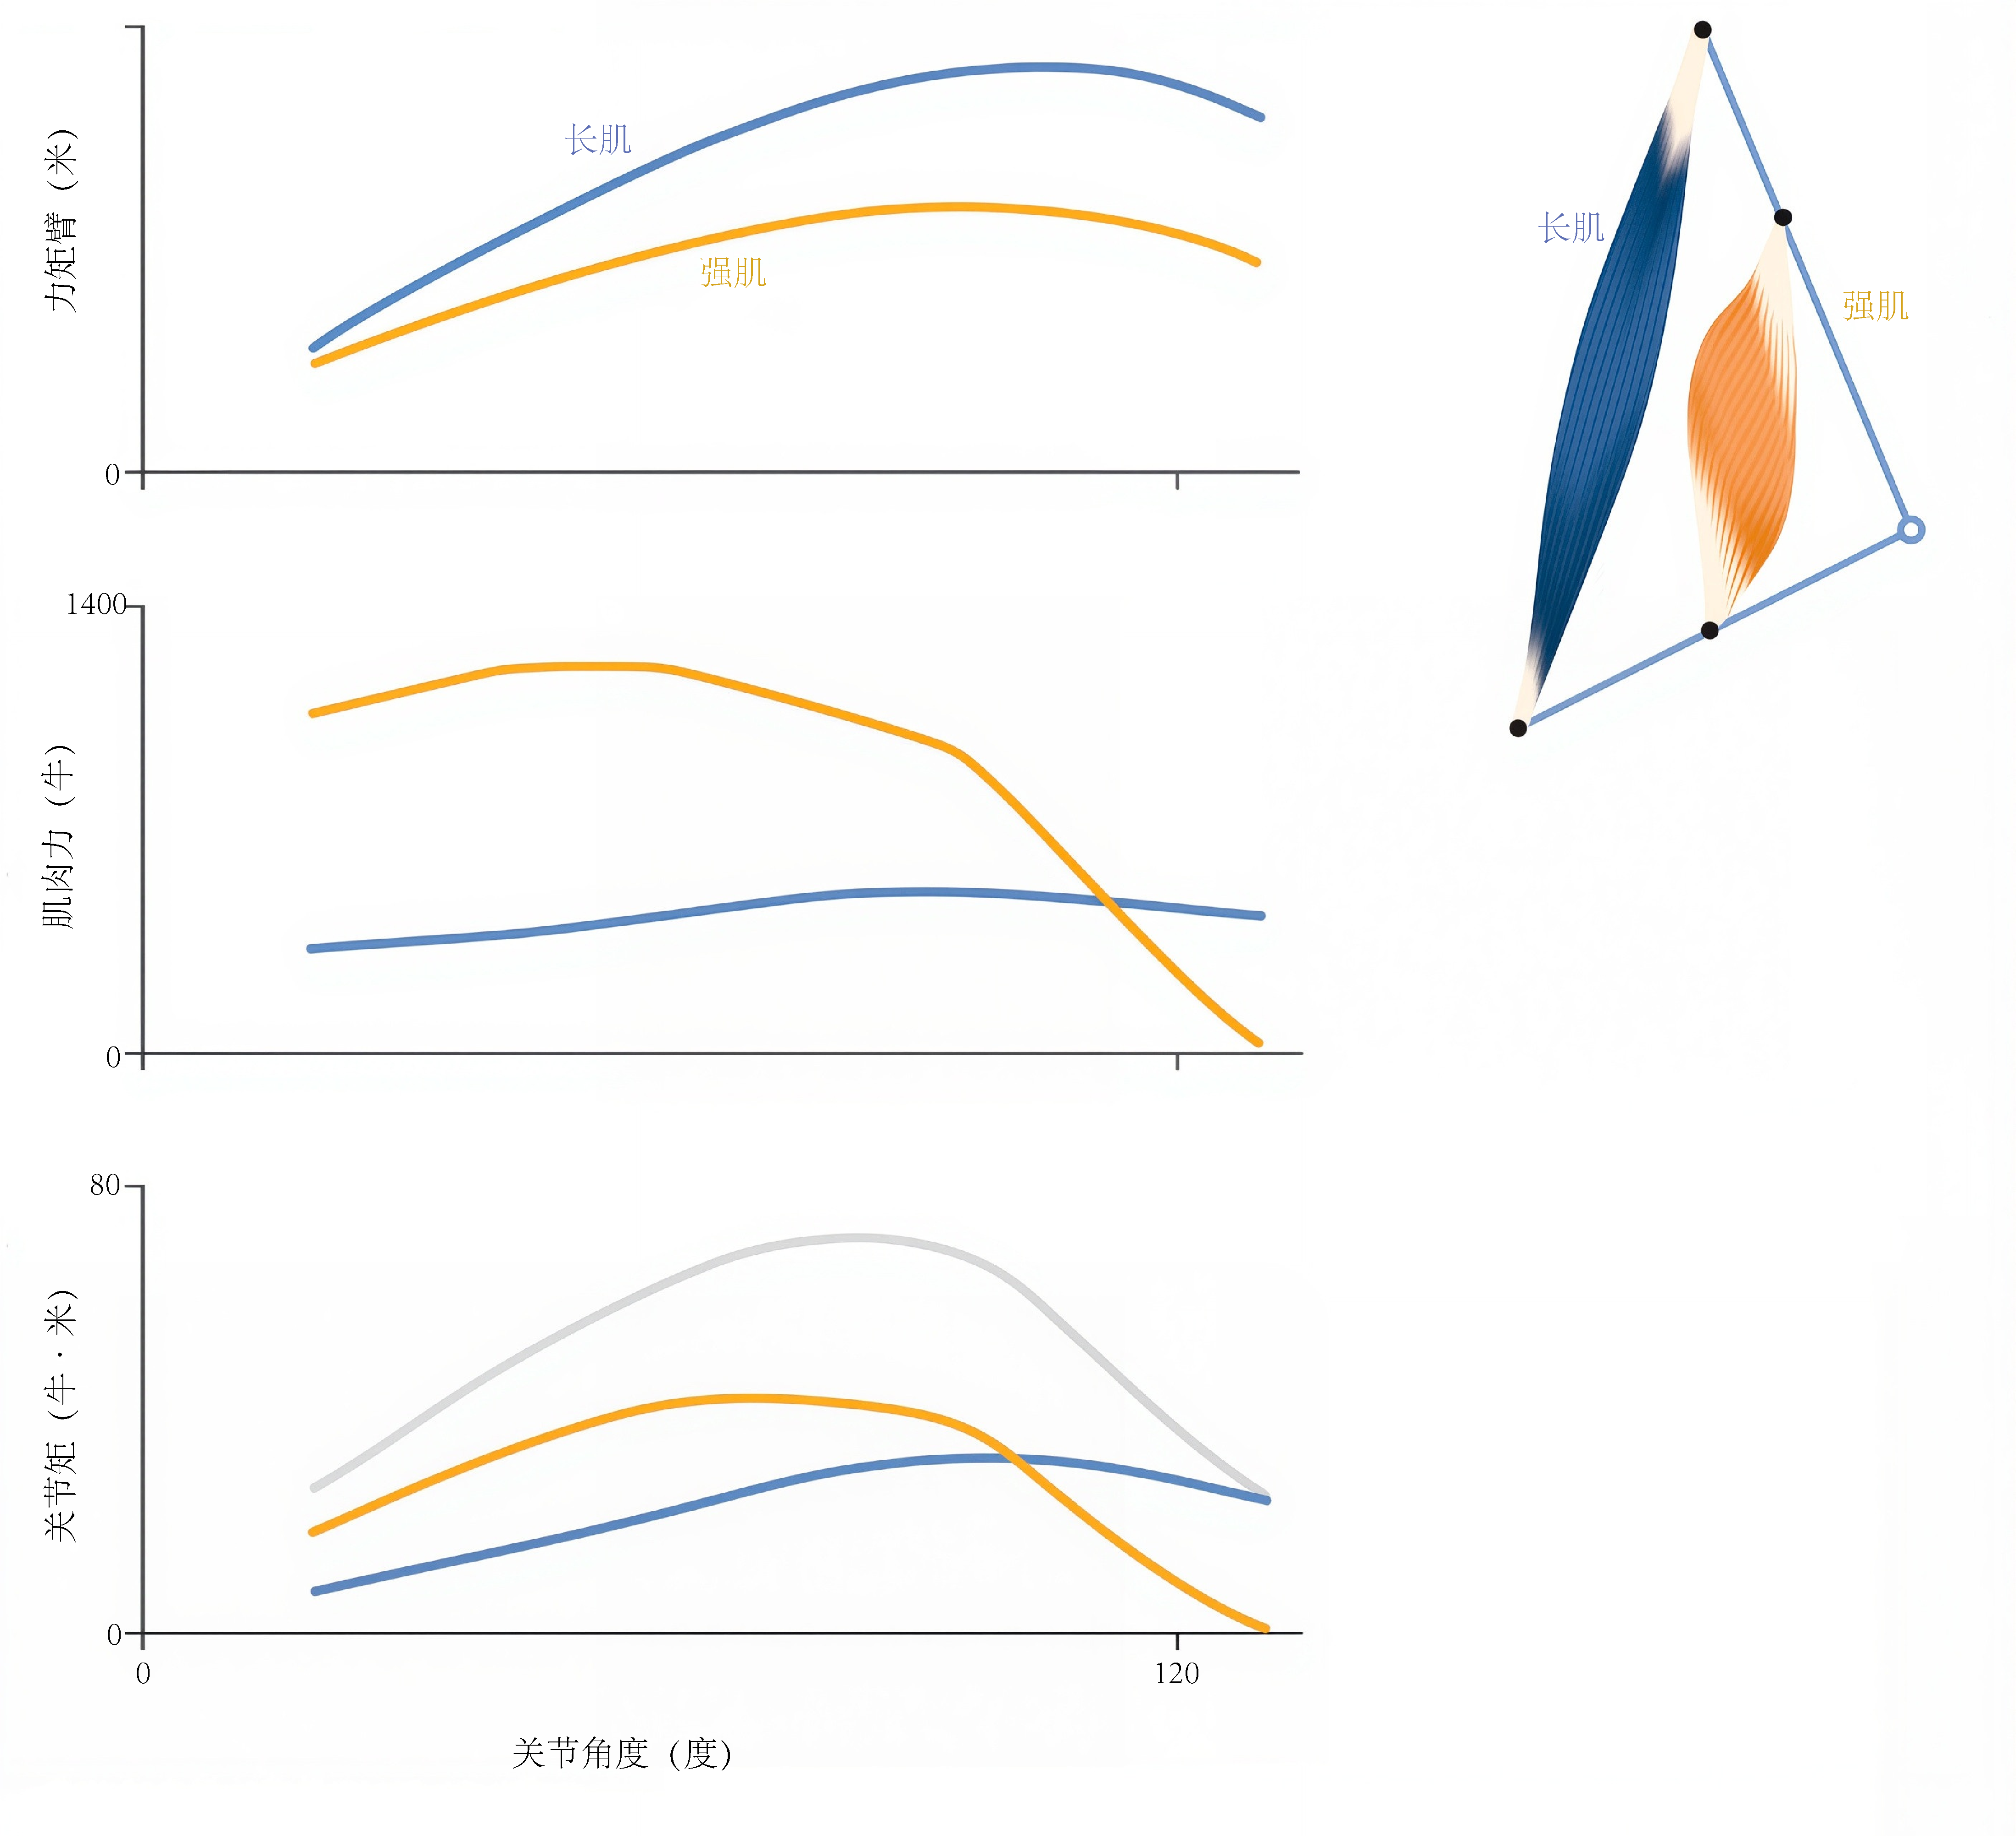
\includegraphics[width=1.0\linewidth]{chap6/6_13}
	\caption{肌肉产生的峰值力矩发生在既不对应于峰值力臂也不对应于峰值力的关节角度处,这里以两块虚拟肌肉为例进行说明。
		肌肉群产生的总关节力矩仅仅是该肌肉群中所有肌肉产生的力矩之和。 \label{fig:6_13}}
\end{figure}



\section{肌肉结构、力臂和肌腱转移手术}

通过分析肌腱移植手术,可以阐明肌肉结构和力臂在决定肌肉功能能力方面相互作用的机制。
这类手术适用于因神经或脊髓损伤而部分肌肉功能丧失的患者。
在某些情况下,可以将功能性肌肉的肌腱重新连接到功能性肌肉的肌腱上,以增强肌肉的力量或活动范围。
这些手术可以使患者恢复瘫痪的身体部位。
例如,可以将功能性肘屈肌移植到瘫痪的腕部或手指肌肉上,以恢复抓握物体的能力。


力矩臂在确定肌肉力矩方面的作用在肌腱转移手术中非常重要,在这种手术中,外科医生选择一种结构已经进化到可以在一个位置发挥作用的肌肉,并修改其力矩臂以实现新的功能。
我们必须考虑肌肉力矩臂的变化将如何影响其在所需运动范围内围绕目标关节产生力和力矩的能力。
图~\ref{fig:6_14}~提供了肌腱转移手术的简化图。
在此示例中,外科医生有两种选择来附着功能肌肉的位置,该肌肉的最大等长力为 1.2 kN,最佳纤维长度为 8 厘米。
如果她选择将肌肉附着到肌肉 A 的肌腱上,新配置的肌肉的平均力矩臂将为 4 厘米(蓝色);如果她选择附着点 B,新配置的肌肉的平均力矩臂将为 2 厘米(橙色)。


\begin{figure}[!htb]
	\centering
	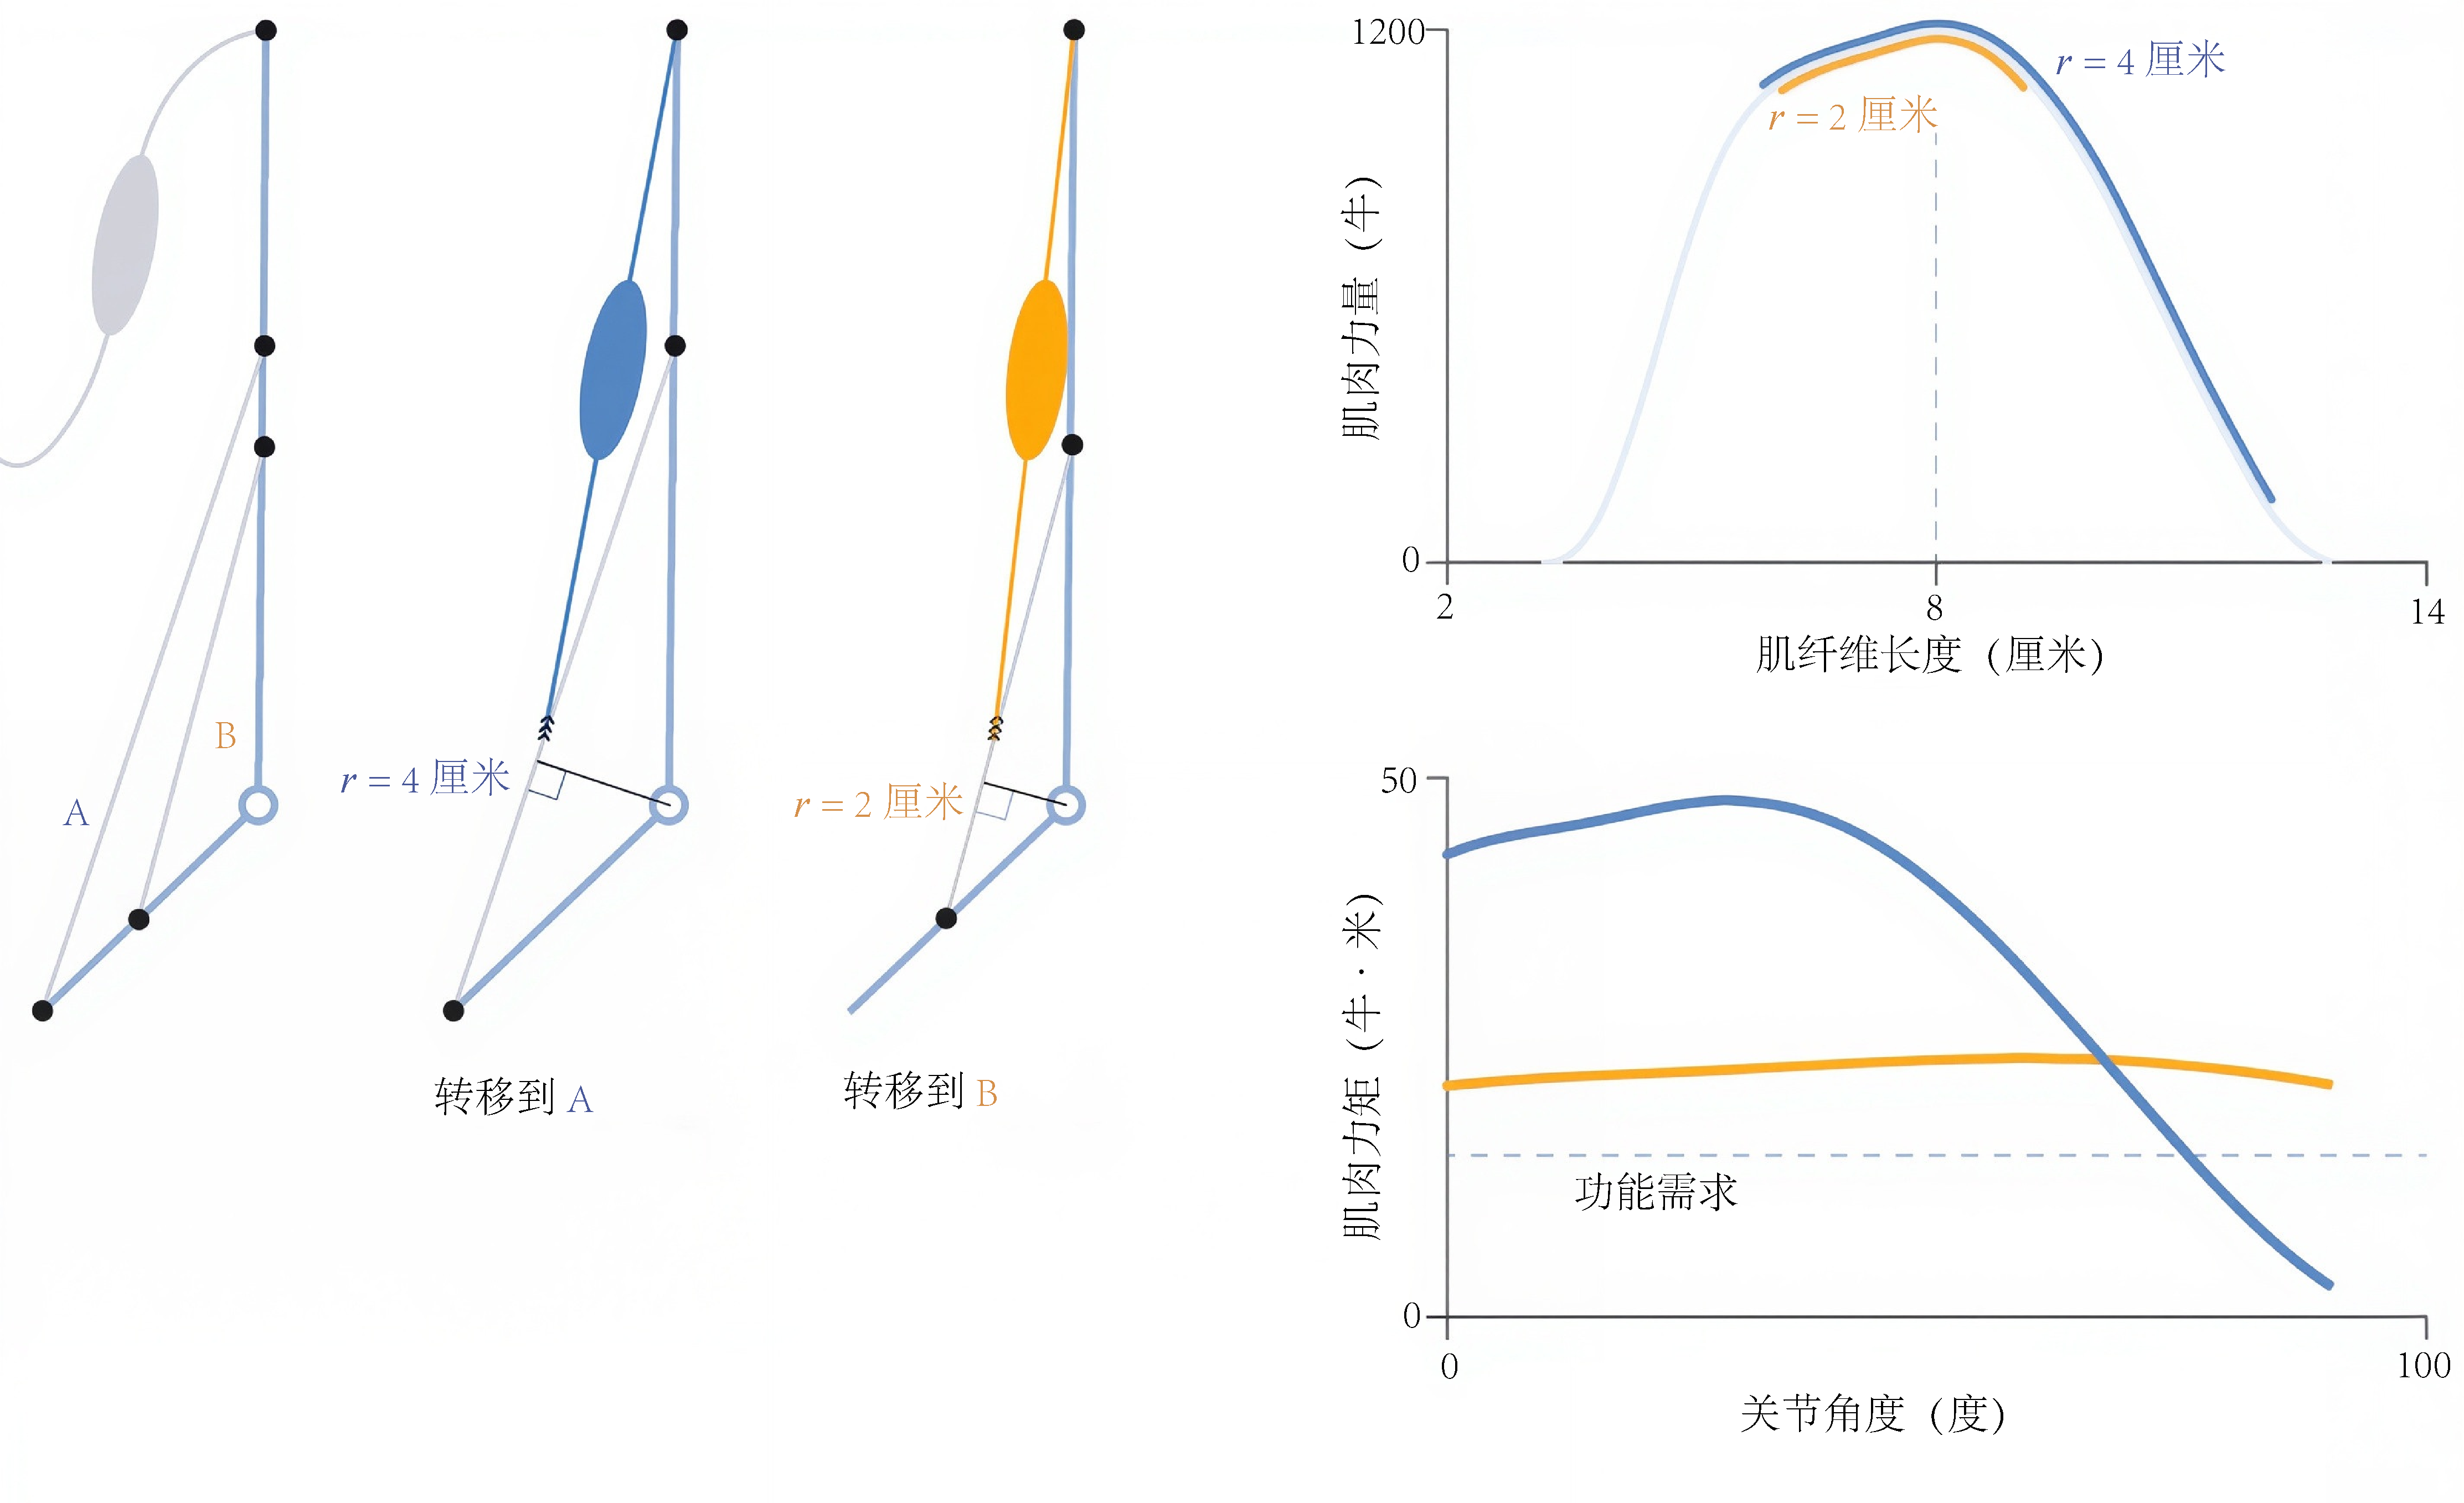
\includegraphics[width=1.0\linewidth]{chap6/6_14}
	\caption{肌肉力和力臂概念在肌腱移植手术决策中的应用。
		在本例中,移植到肌肉 A 的肌腱会产生更高的峰值力矩,但只有选项 B 才能满足给定的功能要求。 \label{fig:6_14}}
\end{figure}


假设要求是重新布线的肌肉必须能够在 90 度运动范围内产生至少 15 N·m 的力矩。
可以制定这样的要求,以便患者能够实现特定目标,例如在手拿水杯的同时将手放到嘴边。
有趣的是,虽然选项 A 由于力矩臂较大而会产生更高的峰值力矩(48 N·m),但肌肉纤维的长度变化也会更大,因此会穿过更大的主动力-长度曲线区域(图~\ref{fig:6_14},右)。
由于力-长度关系,选项 A 会导致关节角度高于约 76 度时最小力矩低于所需的 15 N·m。
相比之下,选项 B 会导致较低的峰值力矩(24 N·m),但由于力臂较小,肌肉在 90 度运动范围内的长度变化较小。
因此,方案 B 中的力和力矩不会随关节角度发生太大变化,最小力矩约为 21 N·m,远高于要求的 15 N·m。
因此,在这种情况下,连接点 B 将是首选。



\section{动作复杂的肌肉臂}

上述定义描述了理解肌肉力如何产生力矩的实用原理;然而,本章开头描述的假设并不适用于某些关节和肌肉。
在这些情况下,必须使用更复杂的分析方法来考虑肌肉力矩臂。
例如,如果肌肉在收缩时明显隆起,则其力矩臂取决于其主动力。
在这种情况下,我们用于推导肌腱偏移定义的假设不再成立,因此计算$\partial l^{MT} / \partial \theta$将不再反映肌肉作用线到关节中心的垂直距离($r$;公式~\ref{eq:6_9})。
同样,如果关节内存在摩擦力,或者肌肉在关节旋转过程中滑过其他结构,那么肌肉无摩擦且独立的假设就会被违反。
最后,有些关节的旋转轴的位置和方向在运动过程中会发生变化。
在这些情况下,必须相对于瞬时旋转中心计算力矩臂,而瞬时旋转中心会随着关节运动而变化。 
Delp 和 Loan\cite{delp1995graphics}和 Sherman 等人\cite{sherman2013moment}对这些特殊情况及其处理方法进行了更深入的描述。


我们还必须表示具有广泛附着点的肌肉以及包裹(弯曲)骨骼和深层肌肉的肌肉的几何形状。
例如,腰大肌具有复杂的路径,环绕骨盆边缘、髋关节囊和股骨颈(图~\ref{fig:6_15})。
此类肌肉路径可以在计算机模型中使用“过孔点”(图中的蓝点)或“包裹面”(线框)来表示,这两种方式都可以防止肌肉穿透相邻结构。
然而,定义能够在多个自由度和较大运动范围内稳健工作的过孔点和包裹面非常困难。
臀大肌的建模也非常困难,因为它具有广泛的附着区域,并且其纤维具有复杂的几何排列。
如图~\ref{fig:6_15}~所示,为了更好地模拟其力学功能,可以将该肌肉分为 3 个肌腱区。
过孔点和包裹面的替代方法是用数十或数百条路径来表示三维纤维几何形状(图~\ref{fig:6_16})。
适当的建模复杂度取决于分析目标。
例如,为了估算几何形状相对简单的肌肉产生的总力矩,如图~\ref{fig:6_6}~所示的模型可能就足够了。
相反,为了计算肌肉内纤维长度的变化如何影响其产力能力,可能需要如图~\ref{fig:6_16}~所示的更详细的模型。


\begin{figure}[!htb]
	\centering
	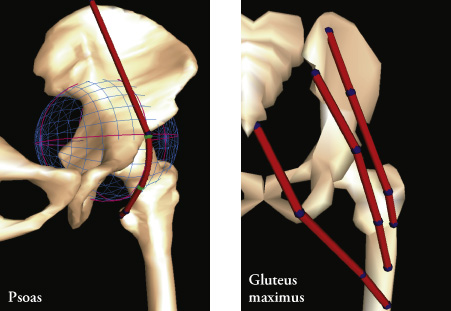
\includegraphics[width=0.7\linewidth]{chap6/6_15}
	\caption{腰大肌包裹骨盆边缘(左图)及臀大肌分离成三个区域(右图)的示意图\cite{blemker2005three}。 \label{fig:6_15}}
\end{figure}


\begin{figure}[!htb]
	\centering
	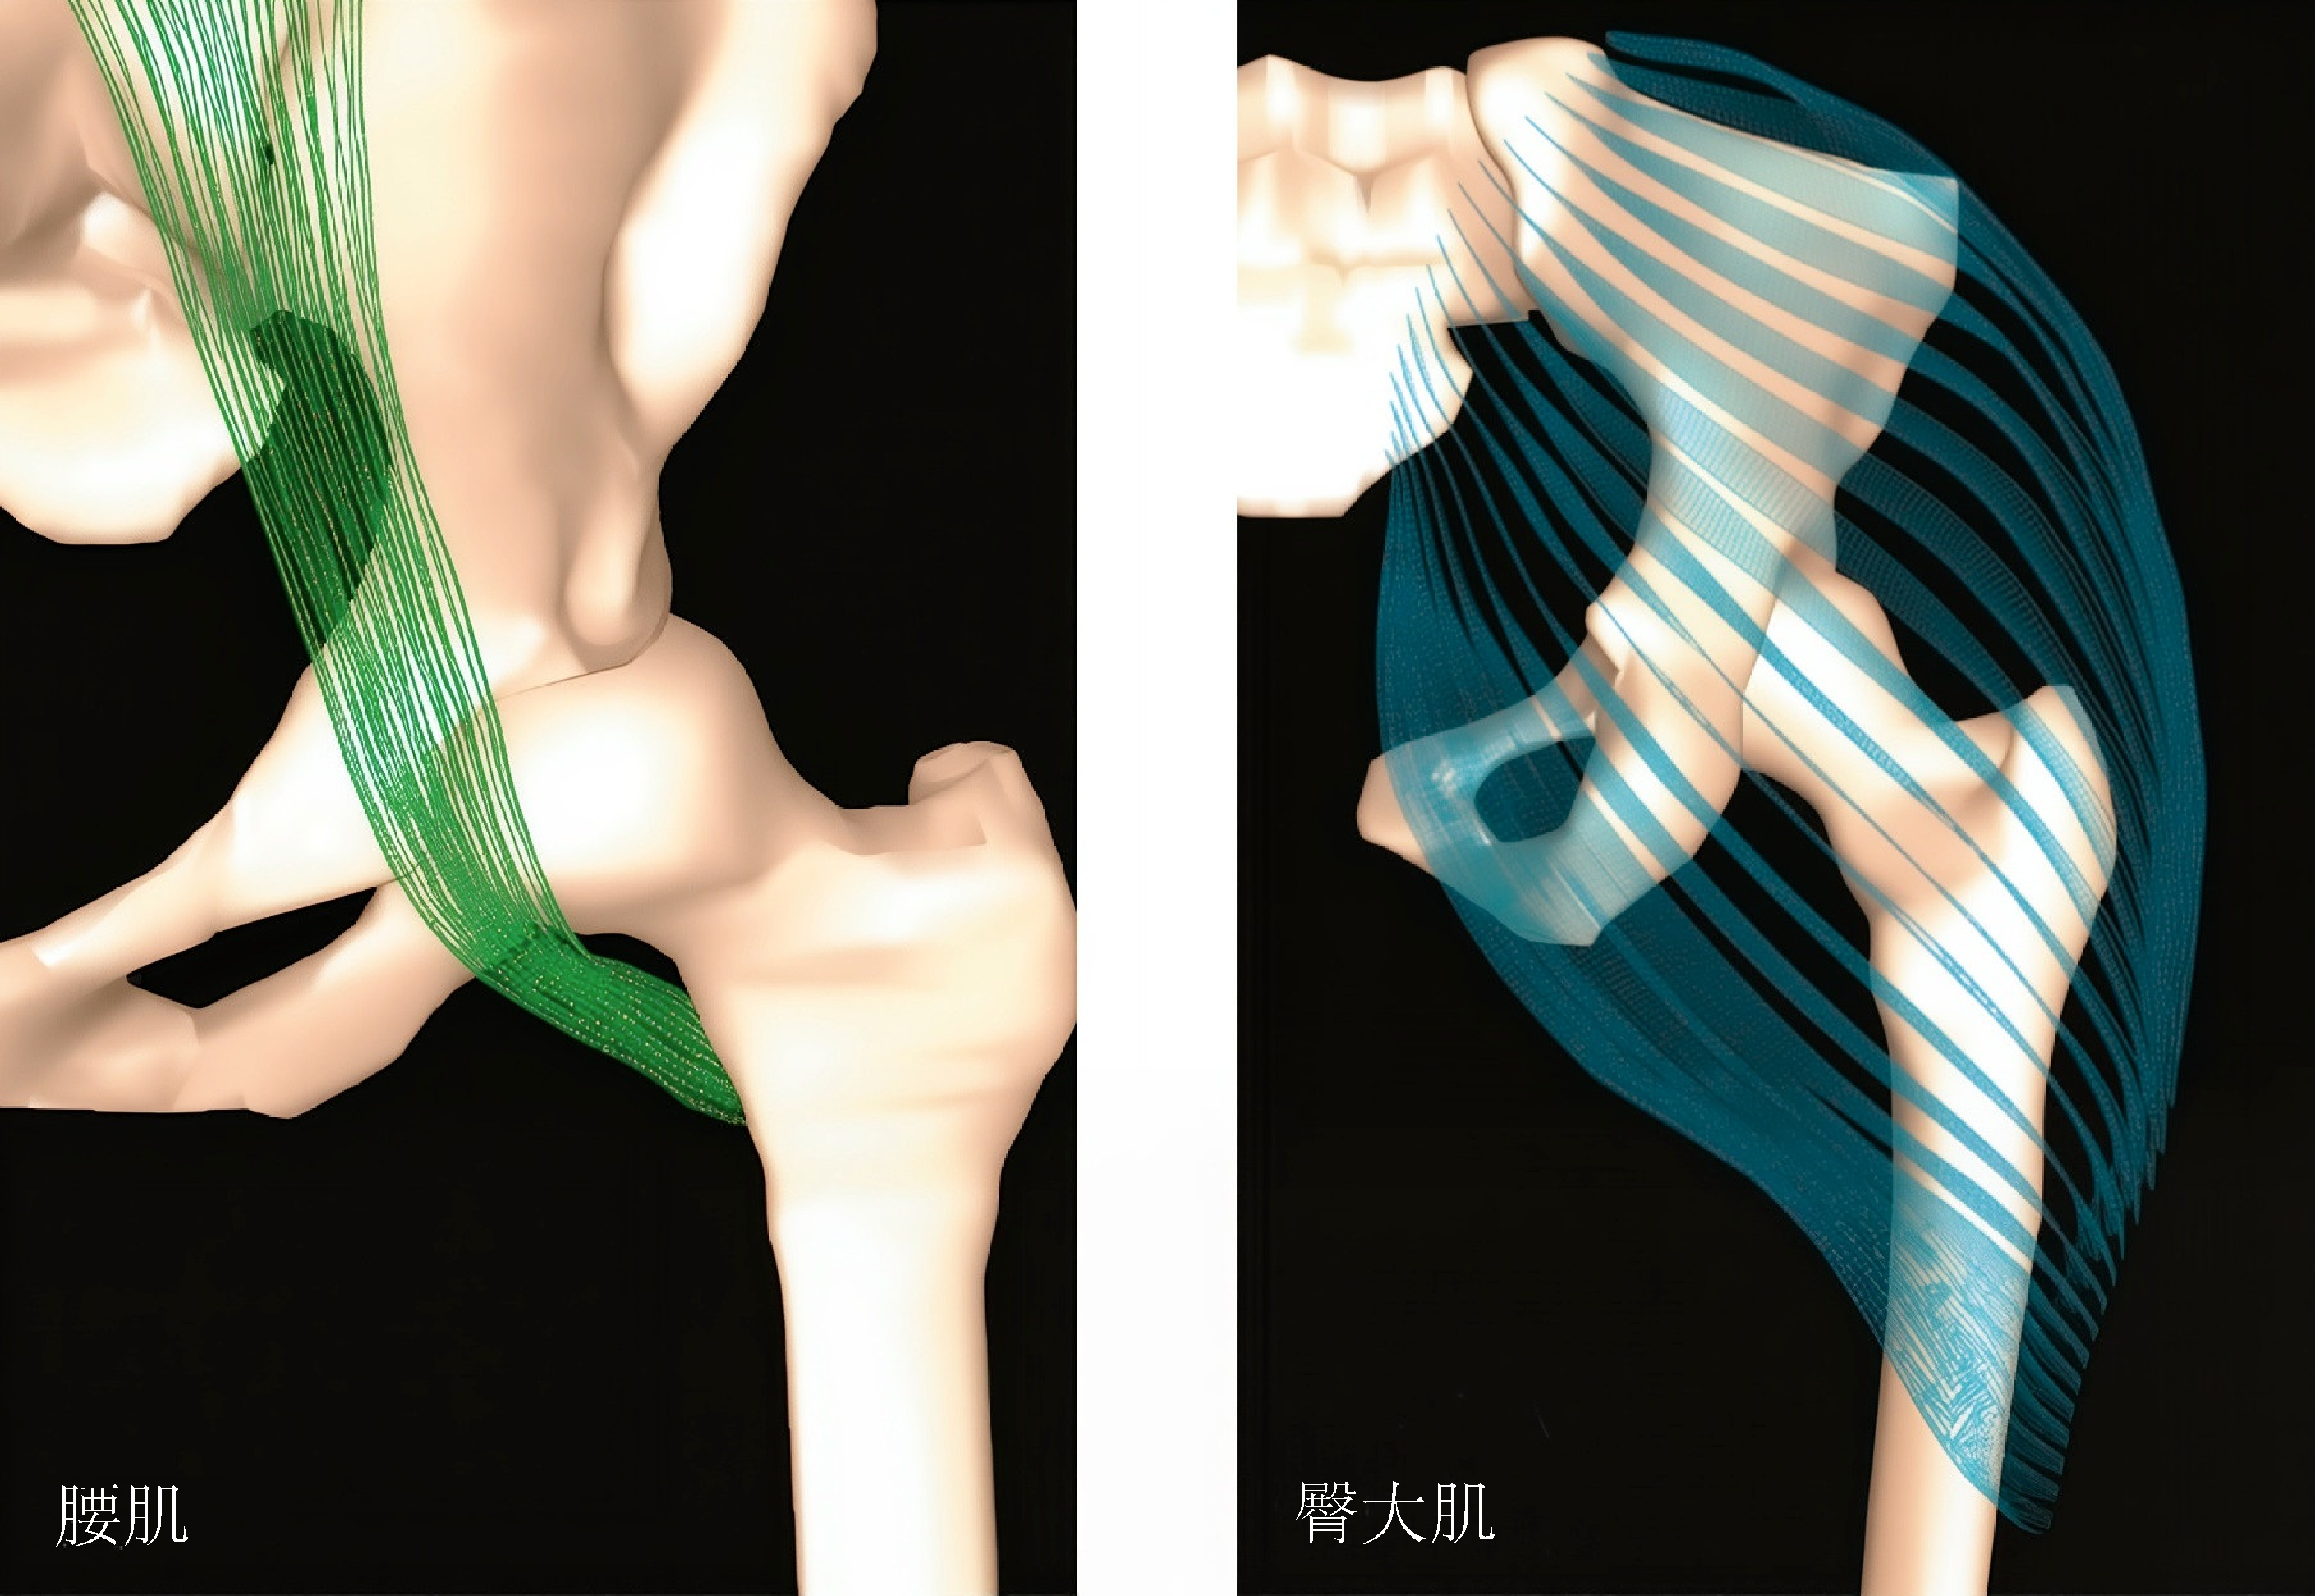
\includegraphics[width=0.7\linewidth]{chap6/6_16}
	\caption{腰大肌(左)和臀大肌(右)的纤维几何结构示意图,有助于详细建模肌肉几何结构和力量的产生\cite{blemker2005three}。 \label{fig:6_16}}
\end{figure}


\section{总结}

我们已经了解了肌肉的力臂如何影响其产生力和关节力矩的能力。
到目前为止,我们假设肌肉处于最大激活状态,就像在力量评估过程中一样;然而,肌肉在运动过程中很少达到最大激活状态。
为了估算肌肉在亚最大激活状态下产生的力和力矩,我们可以使用图~\ref{fig:6_17}~所示的流程。
在所示的示例中,肌电图 (EMG) 数据通过实验收集、过滤,并用于驱动激活动力学模型(第~\ref{chap:chap4}~章)。
然后,每次肌肉激活都被用作肌肉收缩动力学模型的输入(第~\ref{chap:chap5}~章)。
收缩动力学模型的其他关键输入——即肌肉-肌腱单元的长度和速度——可以通过测量关节角度和肌肉骨骼系统模型来确定。


\begin{figure}[!htb]
	\centering
	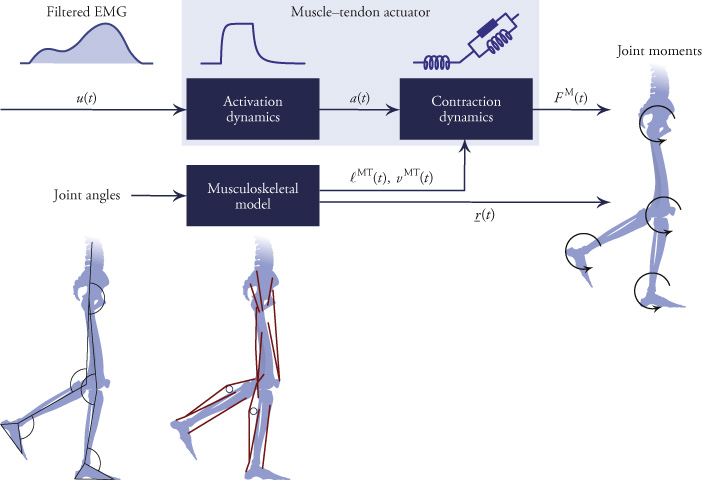
\includegraphics[width=1.0\linewidth]{chap6/6_17}
	\caption{估计肌肉的力量 ($F^M$) 和力臂 ($\underline{r}$) 的过程,用于计算运动过程中肌肉产生的关节力矩。 \label{fig:6_17}}
\end{figure}


图~\ref{fig:6_17}~所示的过程描述了一种正向问题:给定肌电图 (EMG) 数据和关节角度,求出由此产生的肌肉力和关节力矩。
我们将在第~\ref{chap:chap12}~章中运用这一公式来研究跑步过程中肌腱中储存的能量。
生物力学家也经常解决逆向问题,即观察效应,然后使用算法来确定导致这些效应的潜在现象。
例如,我们经常测量身体的运动,并希望估算出产生所观察到的运动所必需的肌肉力。


在接下来的三章中,我们将利用迄今为止所学的知识,探索一些用于逆向分析的工具。
在第~\ref{chap:chap7}~章中,我们将学习如何使用计算模型和算法,通过测量身体各节段的运动来估计关节角度。
第~\ref{chap:chap8}~章将介绍如何利用这些关节角度以及外力测量值来估计净关节力矩。
最后,在第~\ref{chap:chap9}~章中,我们将使用优化方法来估计产生净关节力矩并得出我们计算出的关节轨迹的肌肉力量。
只需通过肌肉骨骼模型的视角观察一些非侵入性测量数据,我们就可以计算出关节内部力量、肌肉活动、能量消耗和其他有价值的信息。



